\renewcommand{\chaptername}{BAB}
%-----------------------------------------------------------------------------%
\chapter{HASIL DAN PEMBAHASAN}
%-----------------------------------------------------------------------------%

\vspace{4.5pt}
\setlength{\parskip}{0.5em}
\section{Perancangan (Design)}\label{sec:bab4_perancangan}
Pada tahan pertama ini peneliti akan melakukan perancangan sebuah infrastruktur dimana sistem Kubernetes dan ArgoCD akan dijalankan lalu
microservice untuk dilakukan simulasi implementasi pada ArgoCD. Semua rancangan akan menggunakan visualisasi diagram secara garis besar (high-level) agar mudah dipahami.

\subsection{Sistem Arsitektur Infrastruktur}
Peneliti menggunakan Proxmox VE (Virtual Environment) yang didalam nya terdapat Virtual Machine berupa Talos OS Linux yang siap digunakan untuk menjalankan Kubernetes cluster
\begin{figure}[H]
    \centering
    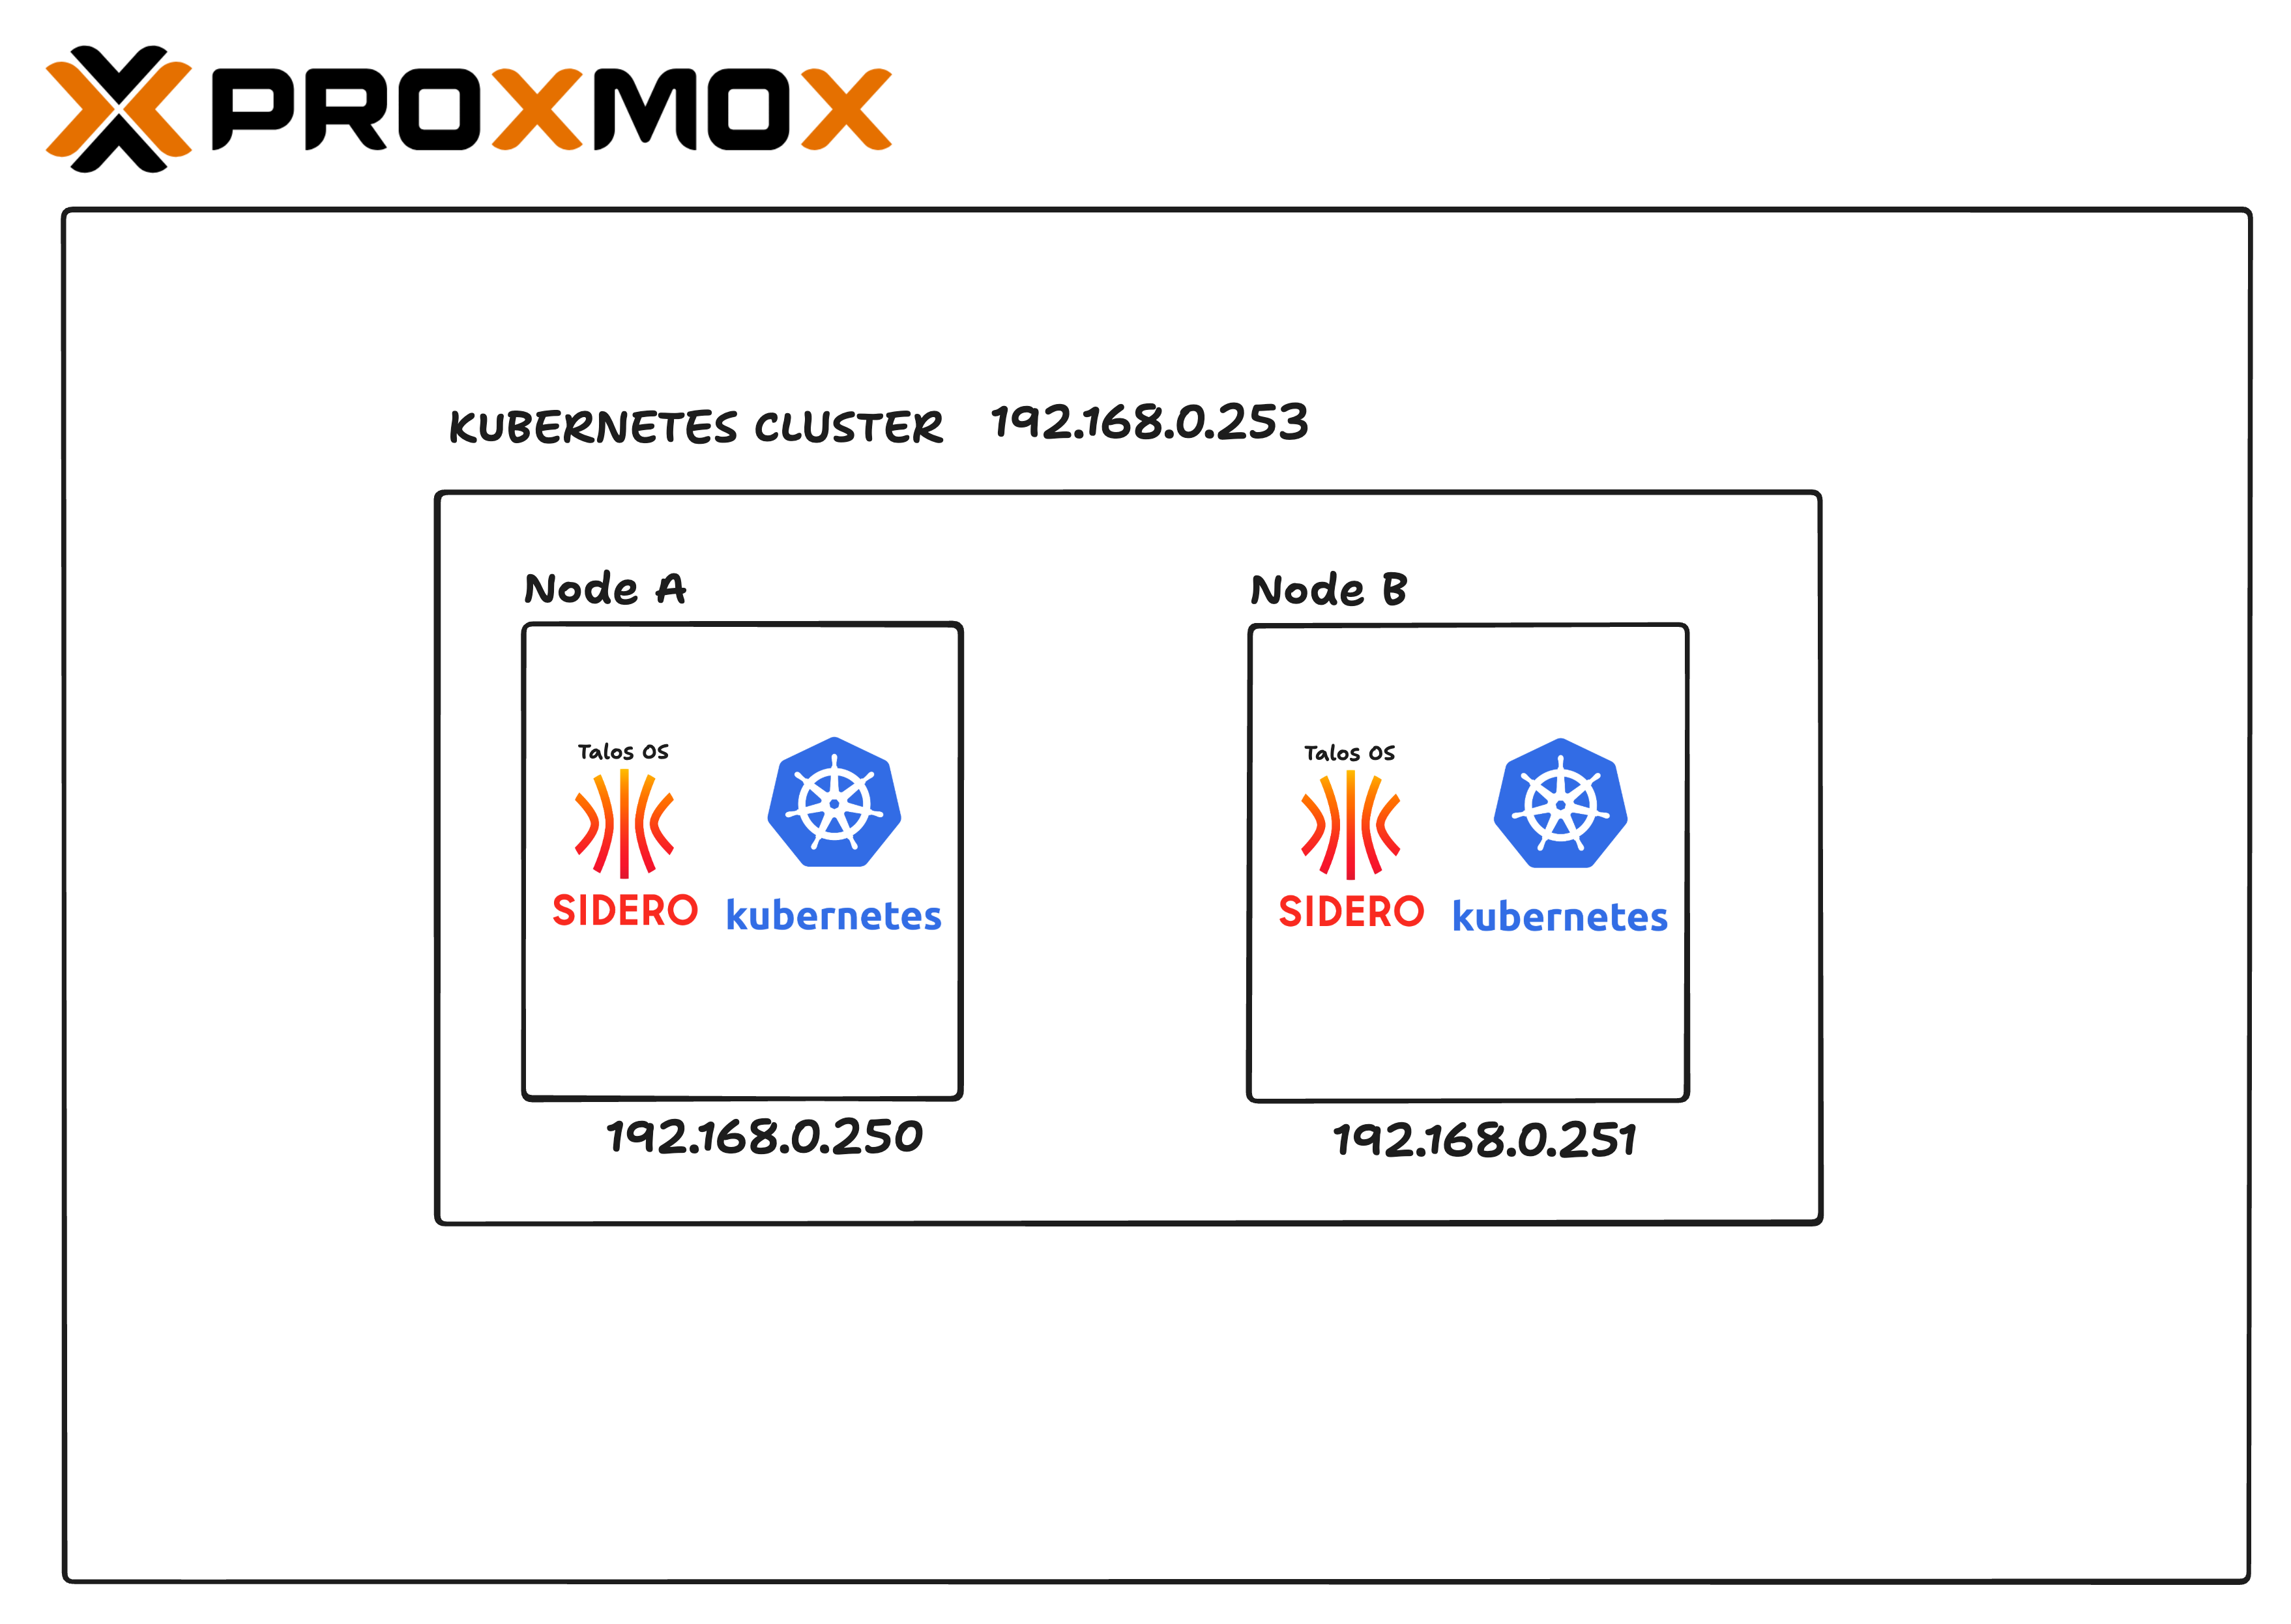
\includegraphics[width=0.9\textwidth]{figures/proxmox-cluster.png}
    \caption{Arsitektur Infrastruktur High Level}
    \label{fig:arsitektur_infrastruktur}
\end{figure}

\subsection{Sistem Arsitektur Kubernetes Cluster}
Pada bagian sebelumnya peneliti sudah memaparkan arsitektur infrastruktur dimana Kubernetes cluster akan berjalan. Pada tahap ini peneliti akan
memaparkan arsitektur pada Kubernetes cluster nya itu sendiri dimana ArgoCD akan berjalan.

\begin{figure}[H]
    \centering
    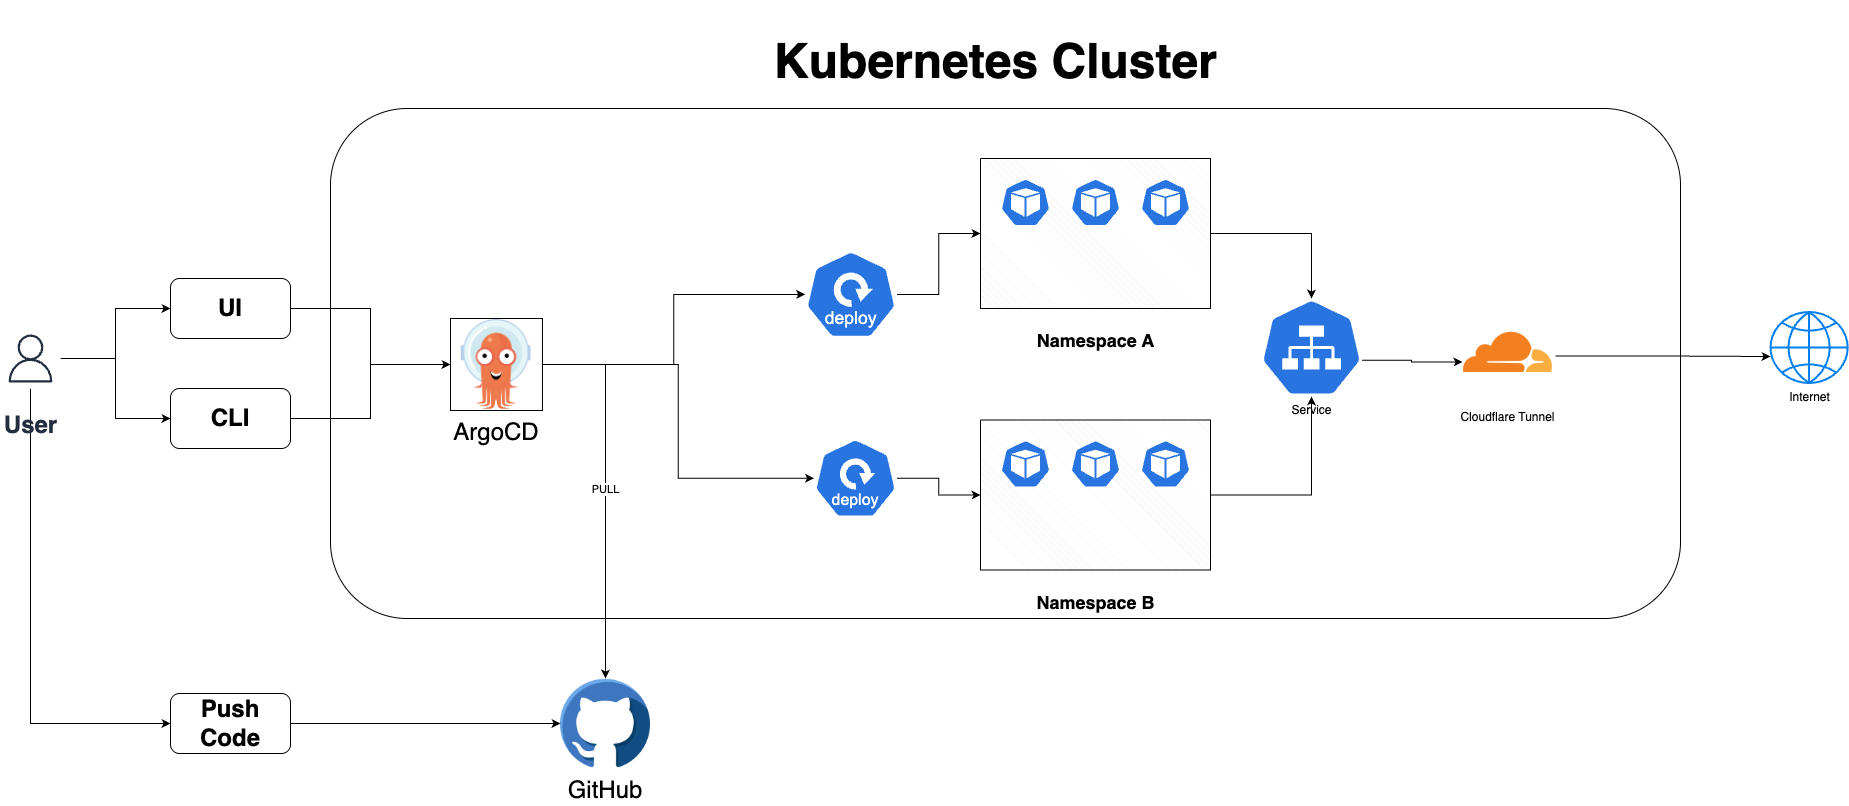
\includegraphics[width=0.9\textwidth]{figures/kube-new.png}
    \caption{Arsitektur Kubernetes High Level}
    \label{fig:arsitektur_kubernetes}
\end{figure}

Didalam sistem Kubernetes cluster yang dibuat terdapat komponen ArgoCD dan Cloudflare Tunnel (optional) yang bertujuan agar server
microservice bisa diakses pada world wide web (internet).

\section{Pengkodean (Coding) / Implementasi}
Tahap ini peneliti akan menjabarkan secara rinci pengkodean/implementasi rancangan sistem yang sudah dirancang.
Peneliti akan melakukan implementasi rancangan sistem menggunakan beberapa komponen yaitu
\begin{enumerate}
    \item Proxmox VE (versi 8.4)
    \item Talos OS (versi 1.9.5)
    \item Kubernetes
    \item ArgoCD
    \item Cloudflare Tunnel
    \item Git repository (GitHub)
\end{enumerate}

\subsection{Implementasi Proxmox VE}
Untuk implementasi Proxmox VE sendiri peneliti melakukan instalasi proxmox pada 2 mesin dengan arsitektur CPU X86.
Pertama kita akan download ISO file atau installer proxmox yang terdapat di link ini \verb|https://enterprise.proxmox.com/iso/proxmox-ve_8.4-1.iso|.
Setelah itu kita memerlukan sebuah Flashdisk atau media untuk bootable ISO tersebut disini peneliti menggunakan tools yang bernama Rufus

\begin{figure}[H]
    \centering
    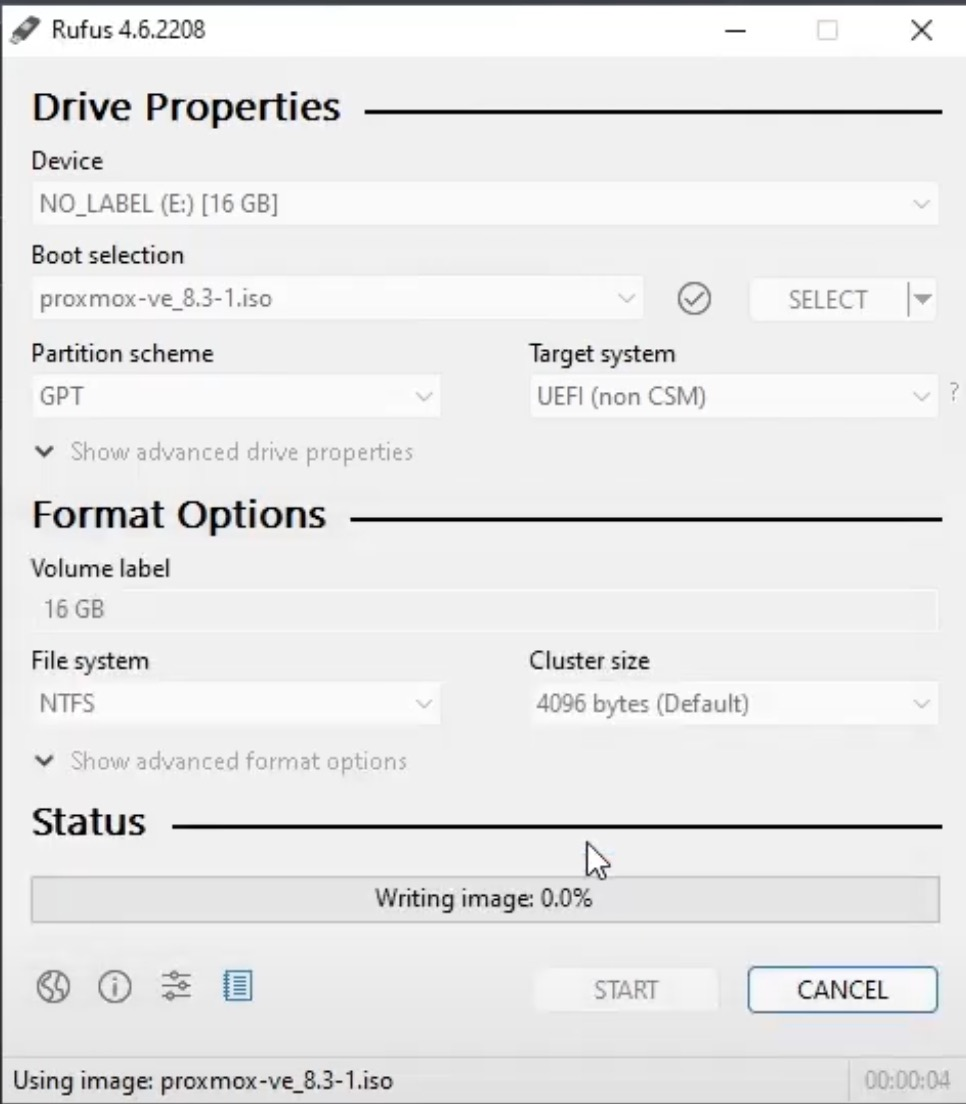
\includegraphics[width=0.8\textwidth]{figures/proxmox-install-rufus-1.jpg}
    \caption{Proses Pembuatan Bootable Proxmox Menggunakan Rufus}
    \label{fig:proxmox_rufus}
\end{figure}

Setelah itu kita perlu mengganti bootable menu yang mengarah pada flashdisk atau media yang kita gunakan untuk instalasi proxmox ketika booting BIOS pada mesin yang digunakan.
Akan terdapat layar instalasi Rufus seperti ini yang akan muncul pada mesin yang kita gunakan.

\begin{figure}[H]
    \centering
    
\includegraphics[width=0.8\textwidth]{figures/proxmox-install-ui-2.jpg}
    \caption{Tampilan Awal Instalasi Proxmox VE}
    \label{fig:proxmox_install_ui}
\end{figure}

Selanjutnya kita tinggal mengikuti apa yang diarahkan secara default oleh user interface yang ditampilkan hingga mesin akan restart dan berada pada tampilan seperti ini.
Pada tampilan layar tersebut terdapat server yang bisa kita gunakan untuk akses user interface melalui browser
\begin{figure}[H]
    \centering
    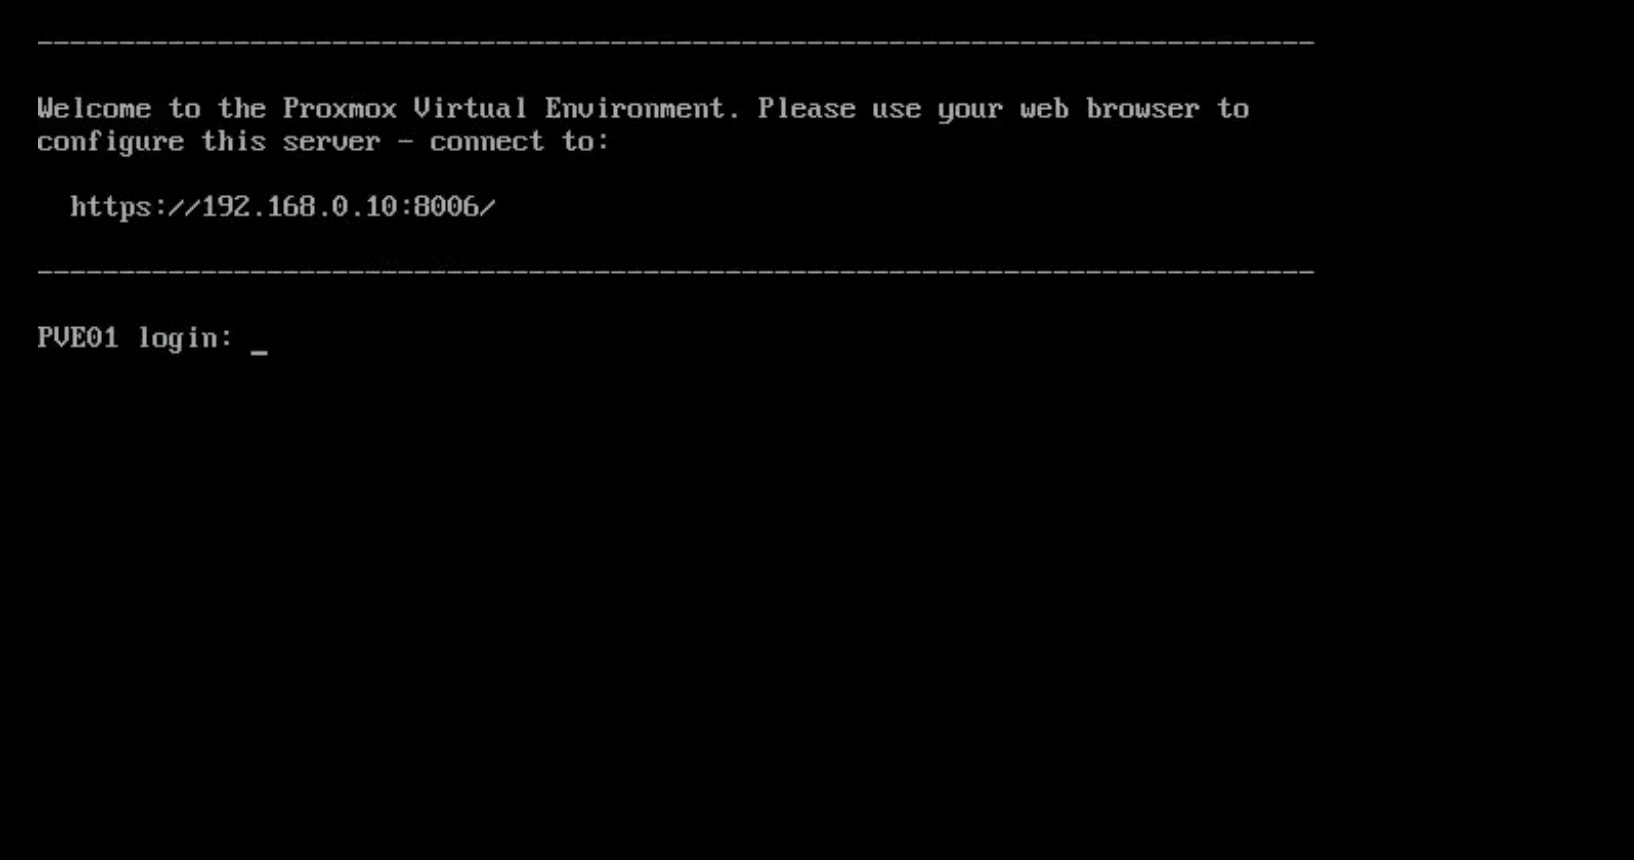
\includegraphics[width=0.8\textwidth]{figures/proxmox-install-terminal-3.jpg}
    \caption{Tampilan Terminal Setelah Instalasi Proxmox Selesai}
    \label{fig:proxmox_terminal}
\end{figure}

Akses UI pada komputer yang ada pada network yang sama dengan Proxmox melalui web user interface.
Peneliti akan mengulang implementasi ini untuk mesin kedua.
\begin{figure}[H]
    \centering
    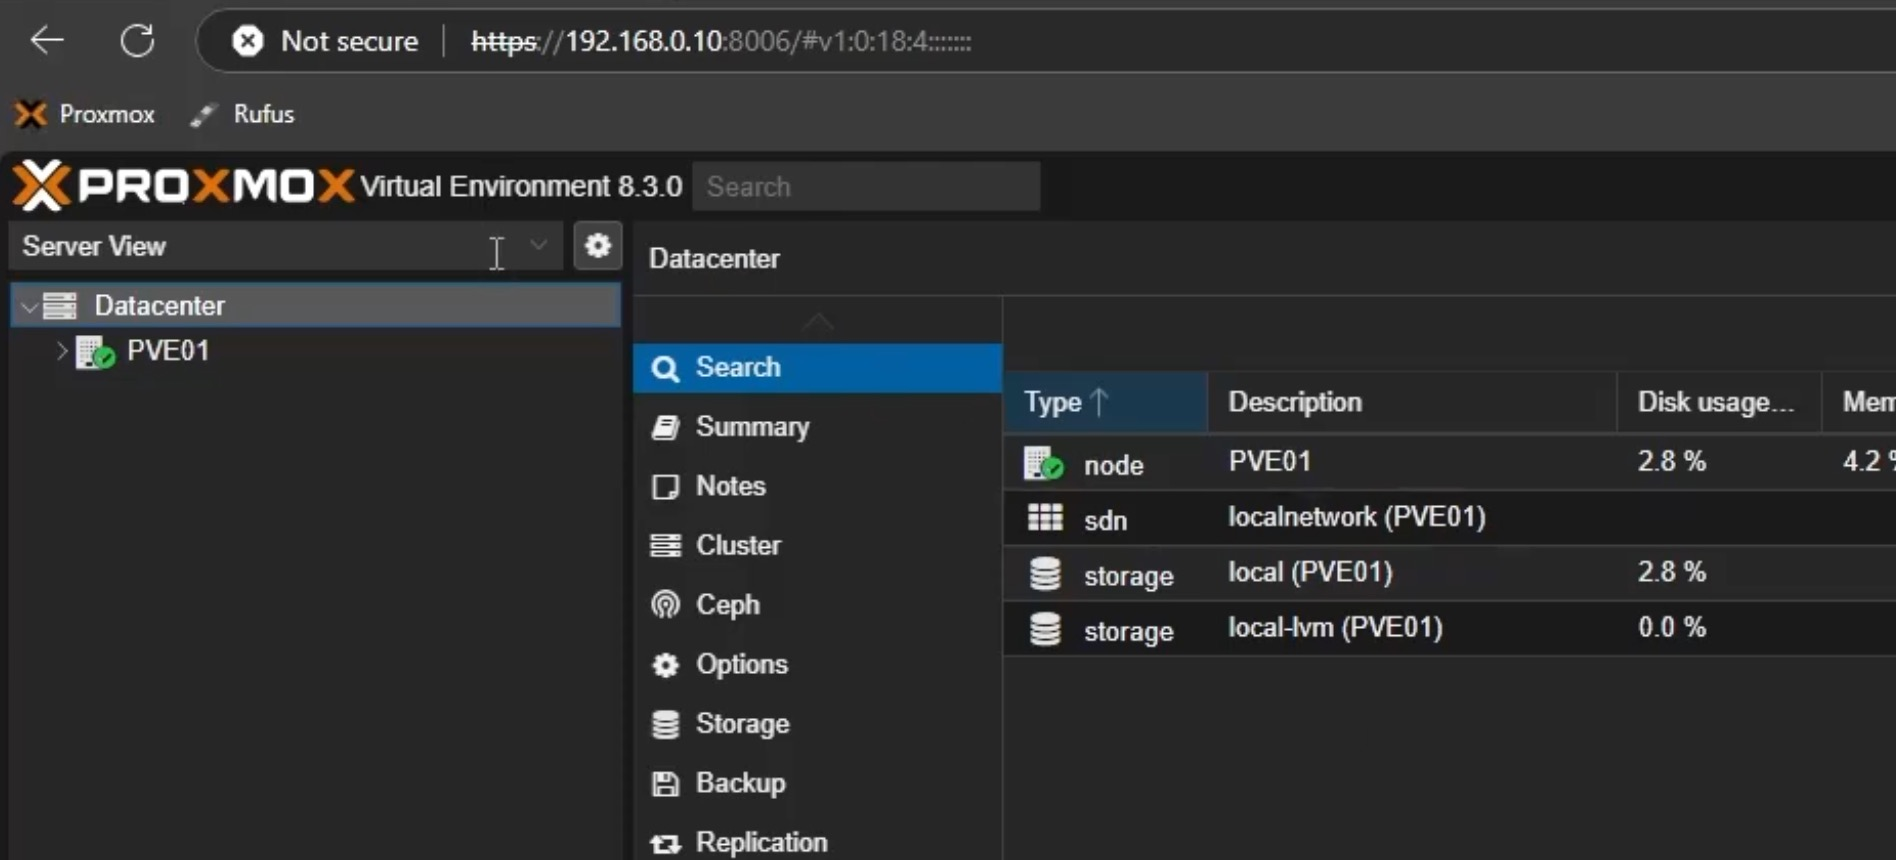
\includegraphics[width=0.9\textwidth]{figures/proxmox-install-web-ui-4.jpg}
    \caption{Tampilan Web Interface Proxmox VE}
    \label{fig:proxmox_webui}
\end{figure}

\subsection{Implementasi Talos OS}
Pada tahap selanjutnya akan dilakukan instalasi Talos OS yang akan di-install menggunakan VM yang ada pada Proxmox VE.
Pertama yang dilakukan adalah mengunduh ISO file Talos OS di sini.

\url{https://github.com/siderolabs/talos/releases/download/v1.9.5/metal-amd64.iso}

\begin{figure}[H]
    \centering
    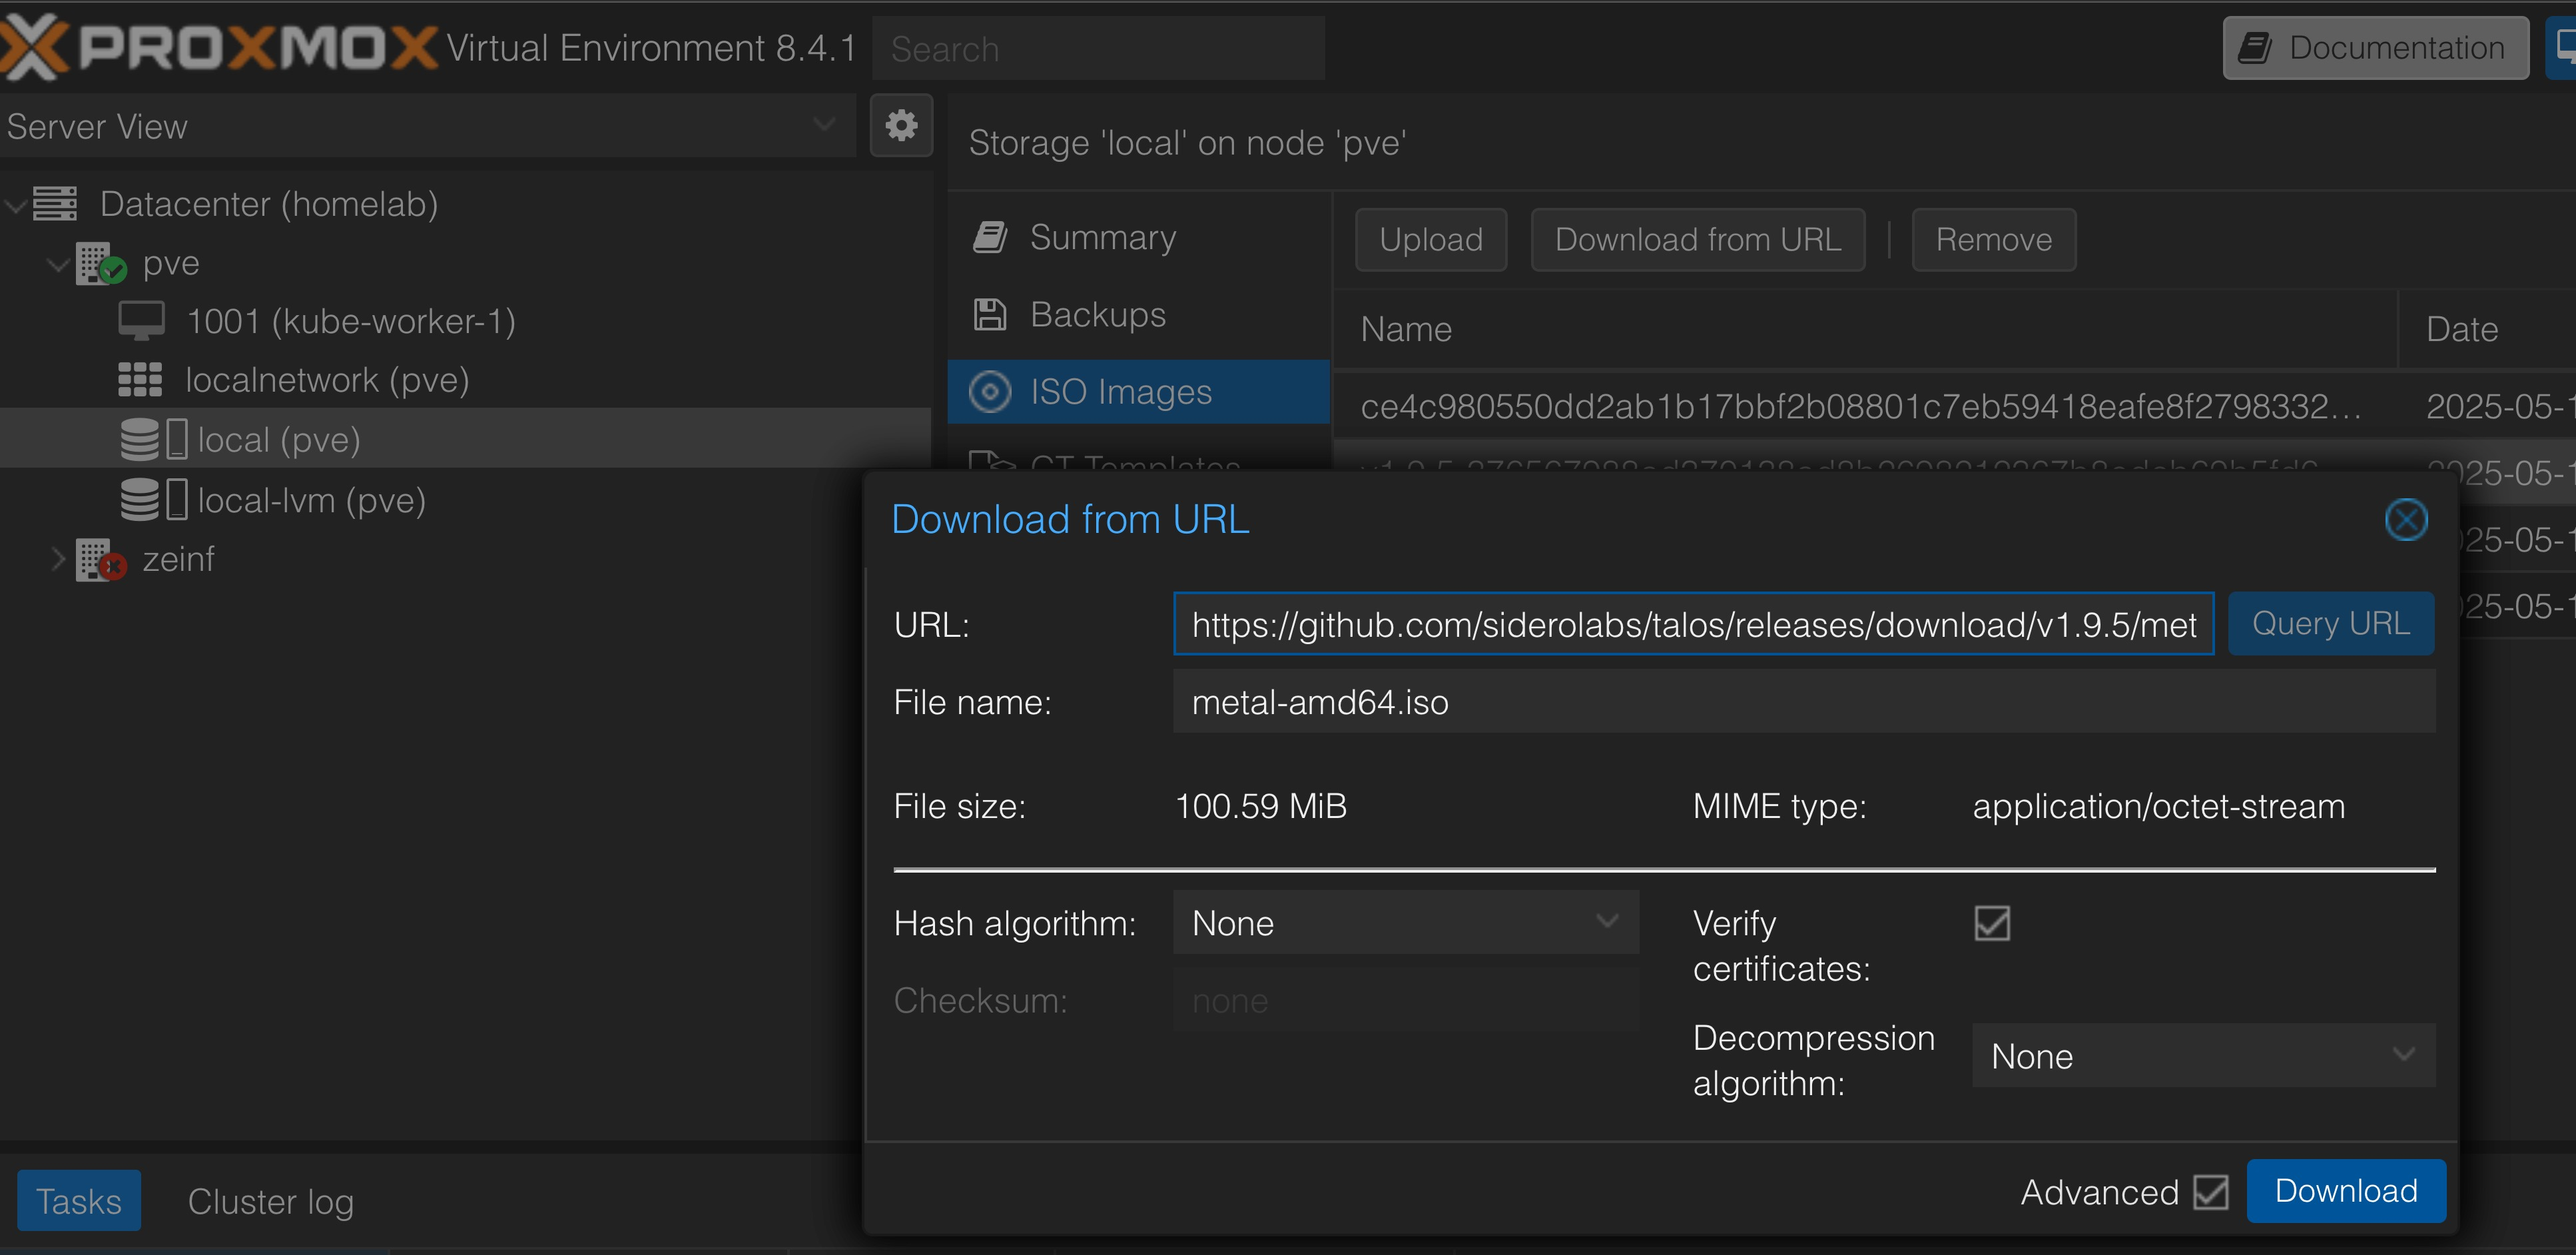
\includegraphics[width=0.8\textwidth]{figures/talos-install-1.jpg}
    \caption{Proses Download ISO Talos OS}
    \label{fig:talos_download}
\end{figure}

Url tersebut lalu didownload melalui proxmox agar tersimpan didalam proxmox. Lalu tahap selanjutnya adalah melakukan instalasi VM Talos OS pada proxmox.

\subsubsection{Instalasi Talos OS}
Tahap ini adalah bagian instalasi VM Talos OS. Peneliti melakukan instalasi pada proxmox VE melalui interface web.
Tahap ini akan dilakukan pada 2 mesin berbeda pada proxmox.

\begin{figure}[!htbp]
    1. Klik Create VM lalu isikan VM ID dan Name untuk VM Talos OS
    \centering
    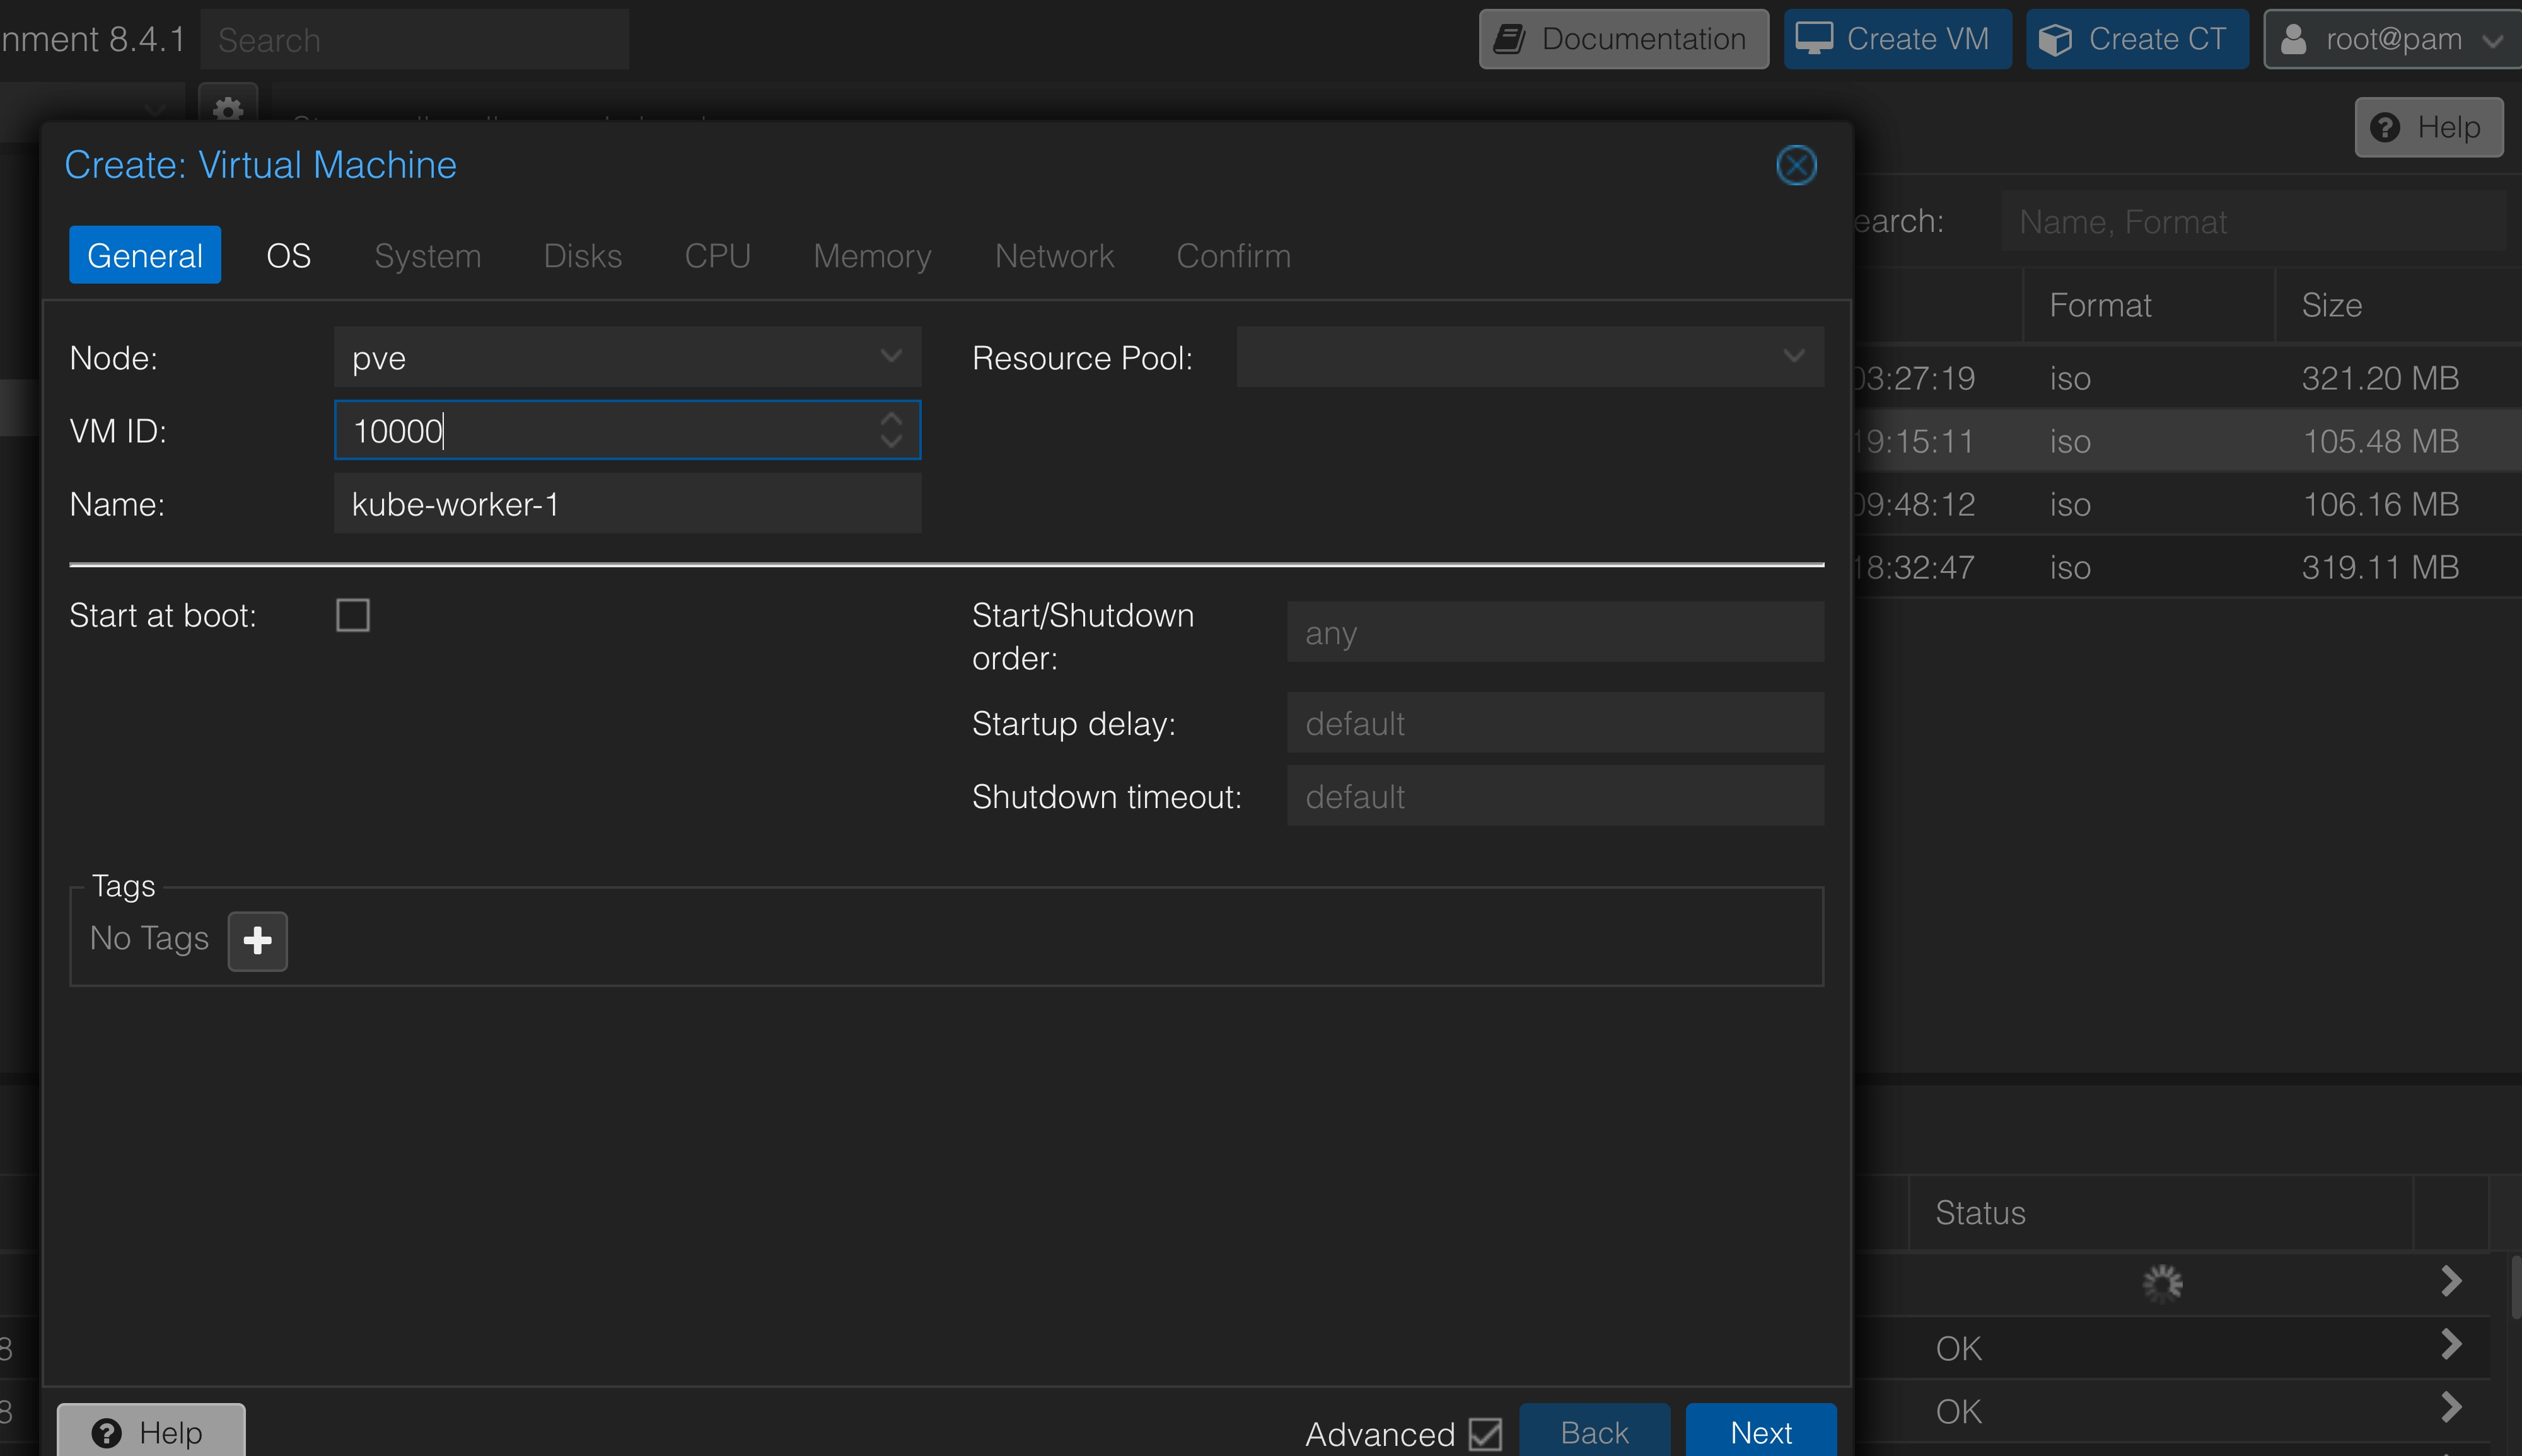
\includegraphics[width=1\textwidth]{figures/talos-install-2.jpg}
    \caption{Instalasi Talos OS 1}
\end{figure}
\begin{figure}[!htbp]
    2. Pada bagian OS. Pilih ISO Talos OS yang baru saja diunduh sebelum nya
    \centering
    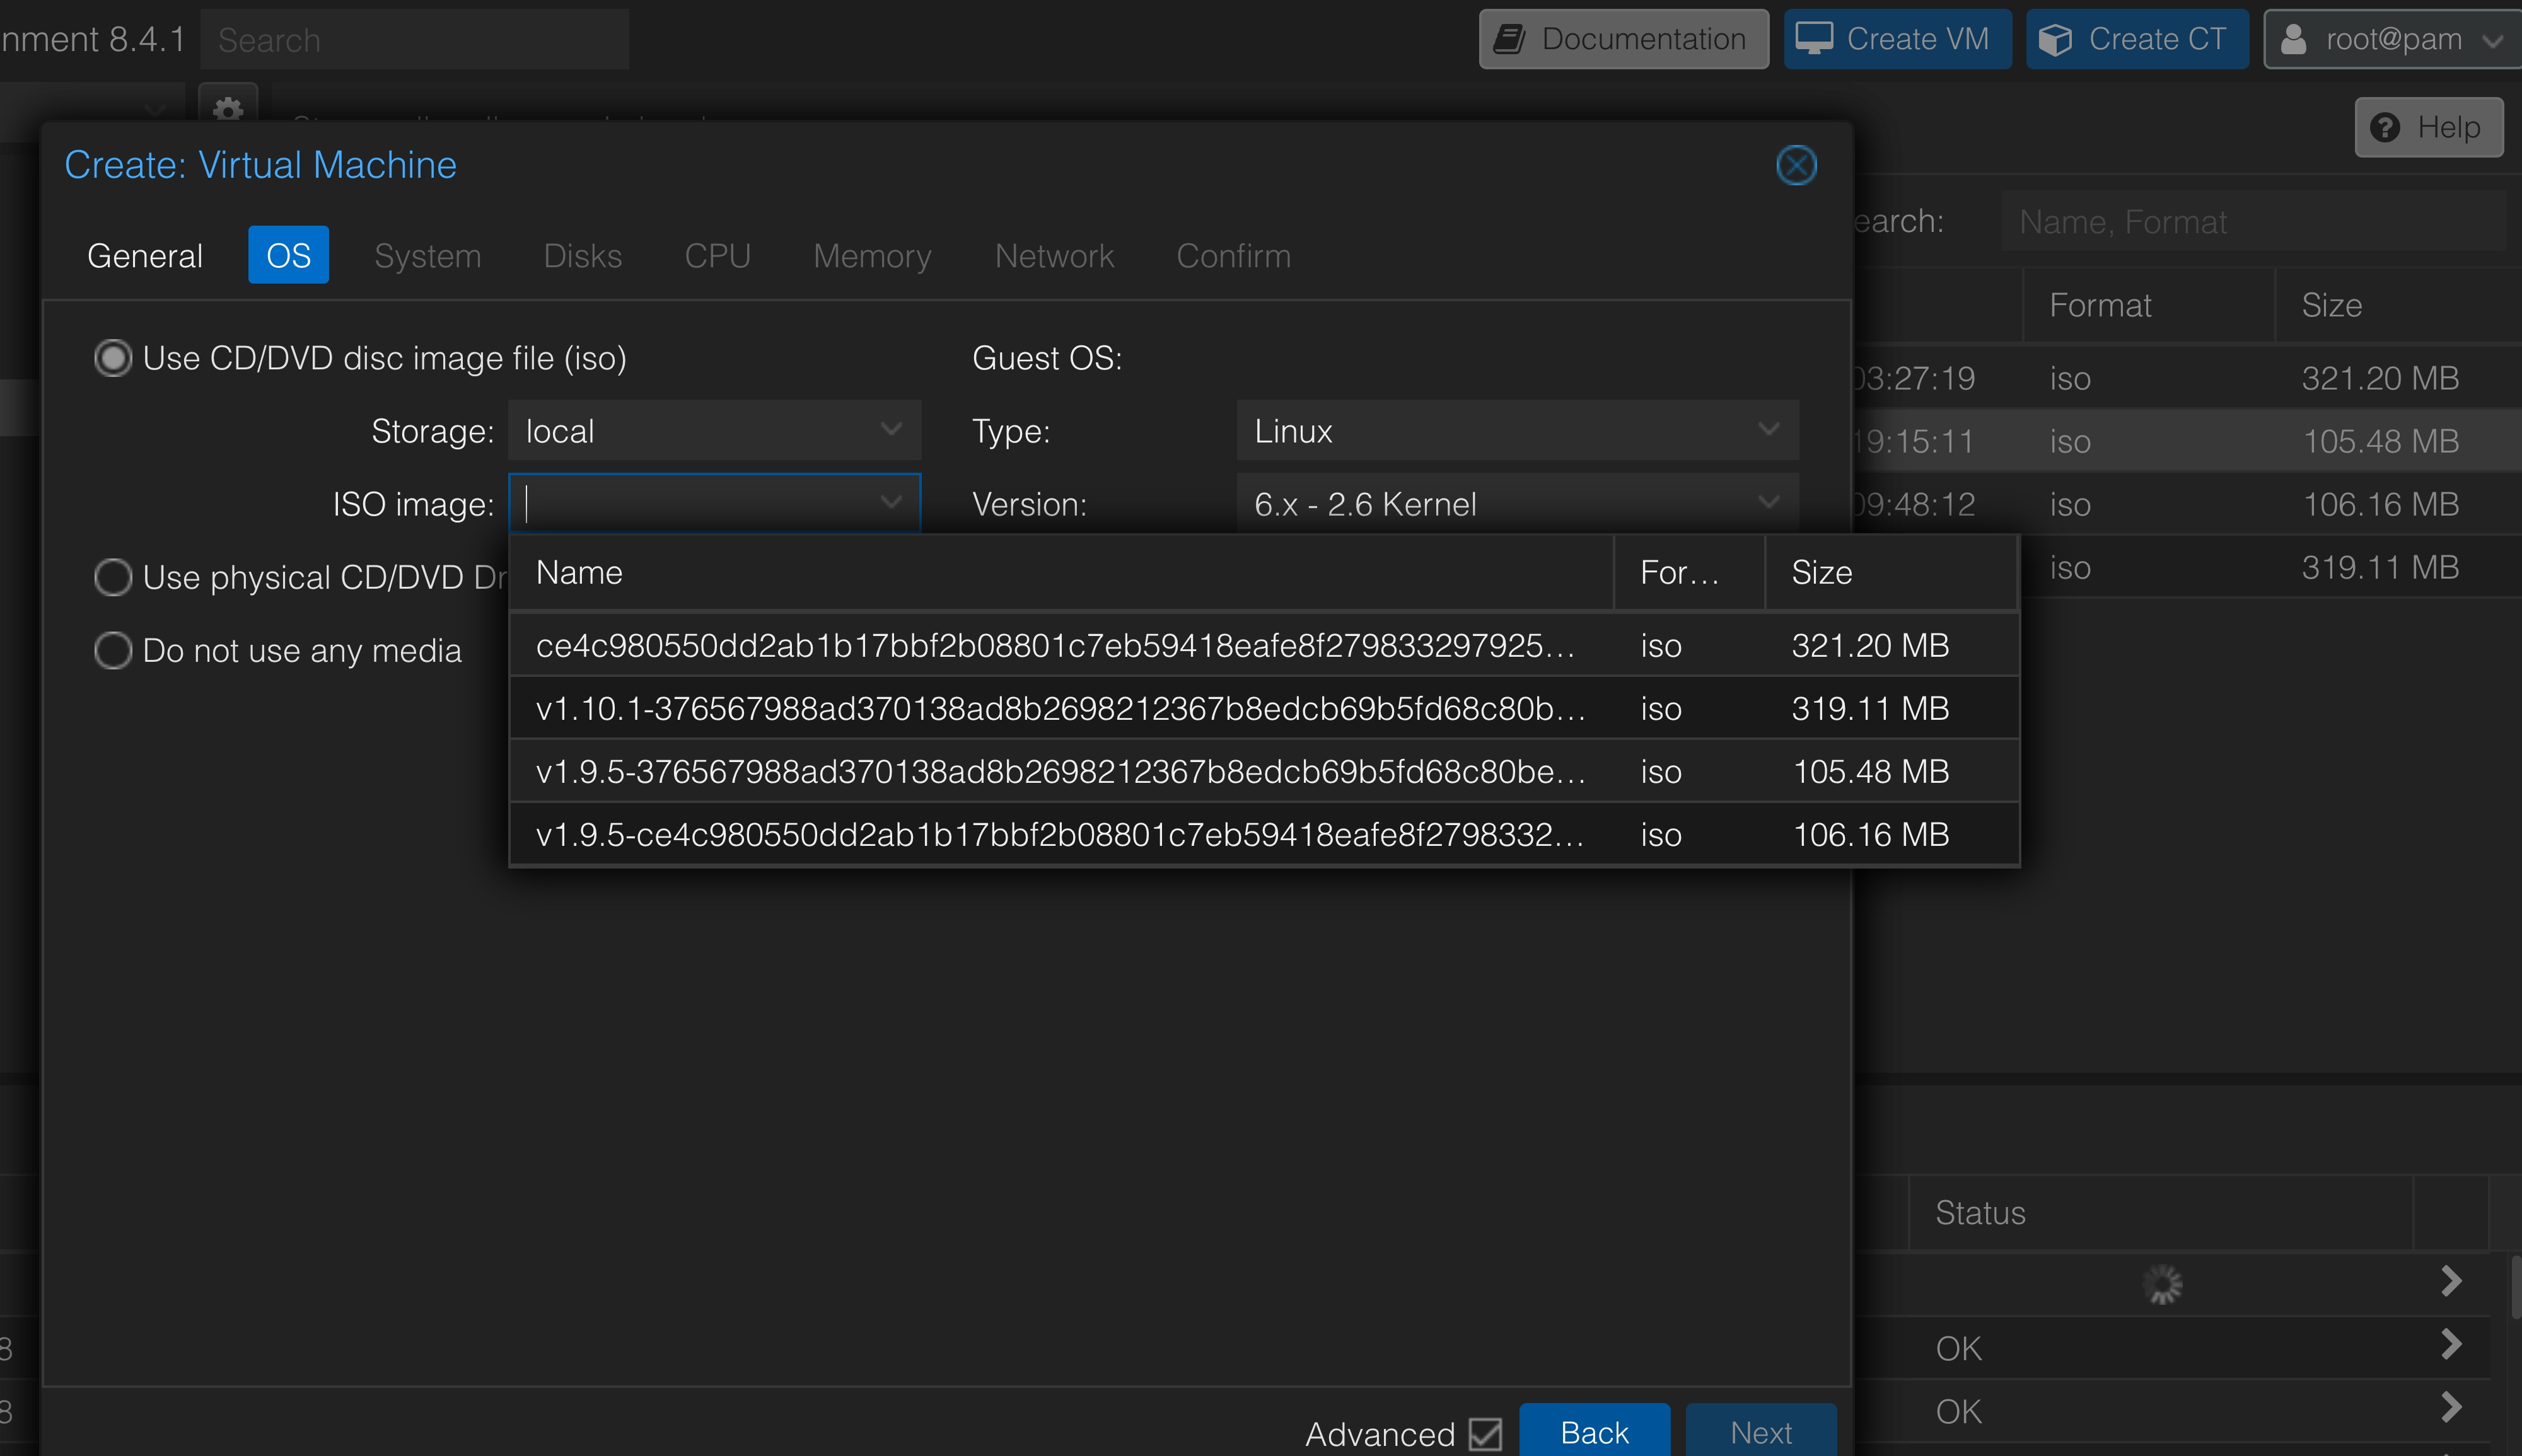
\includegraphics[width=1\textwidth]{figures/talos-install-3.jpg}
    \caption{Instalasi Talos OS 2}
\end{figure}
\begin{figure}[!htbp]
    3. Pada bagian System. cukup next
    \centering
    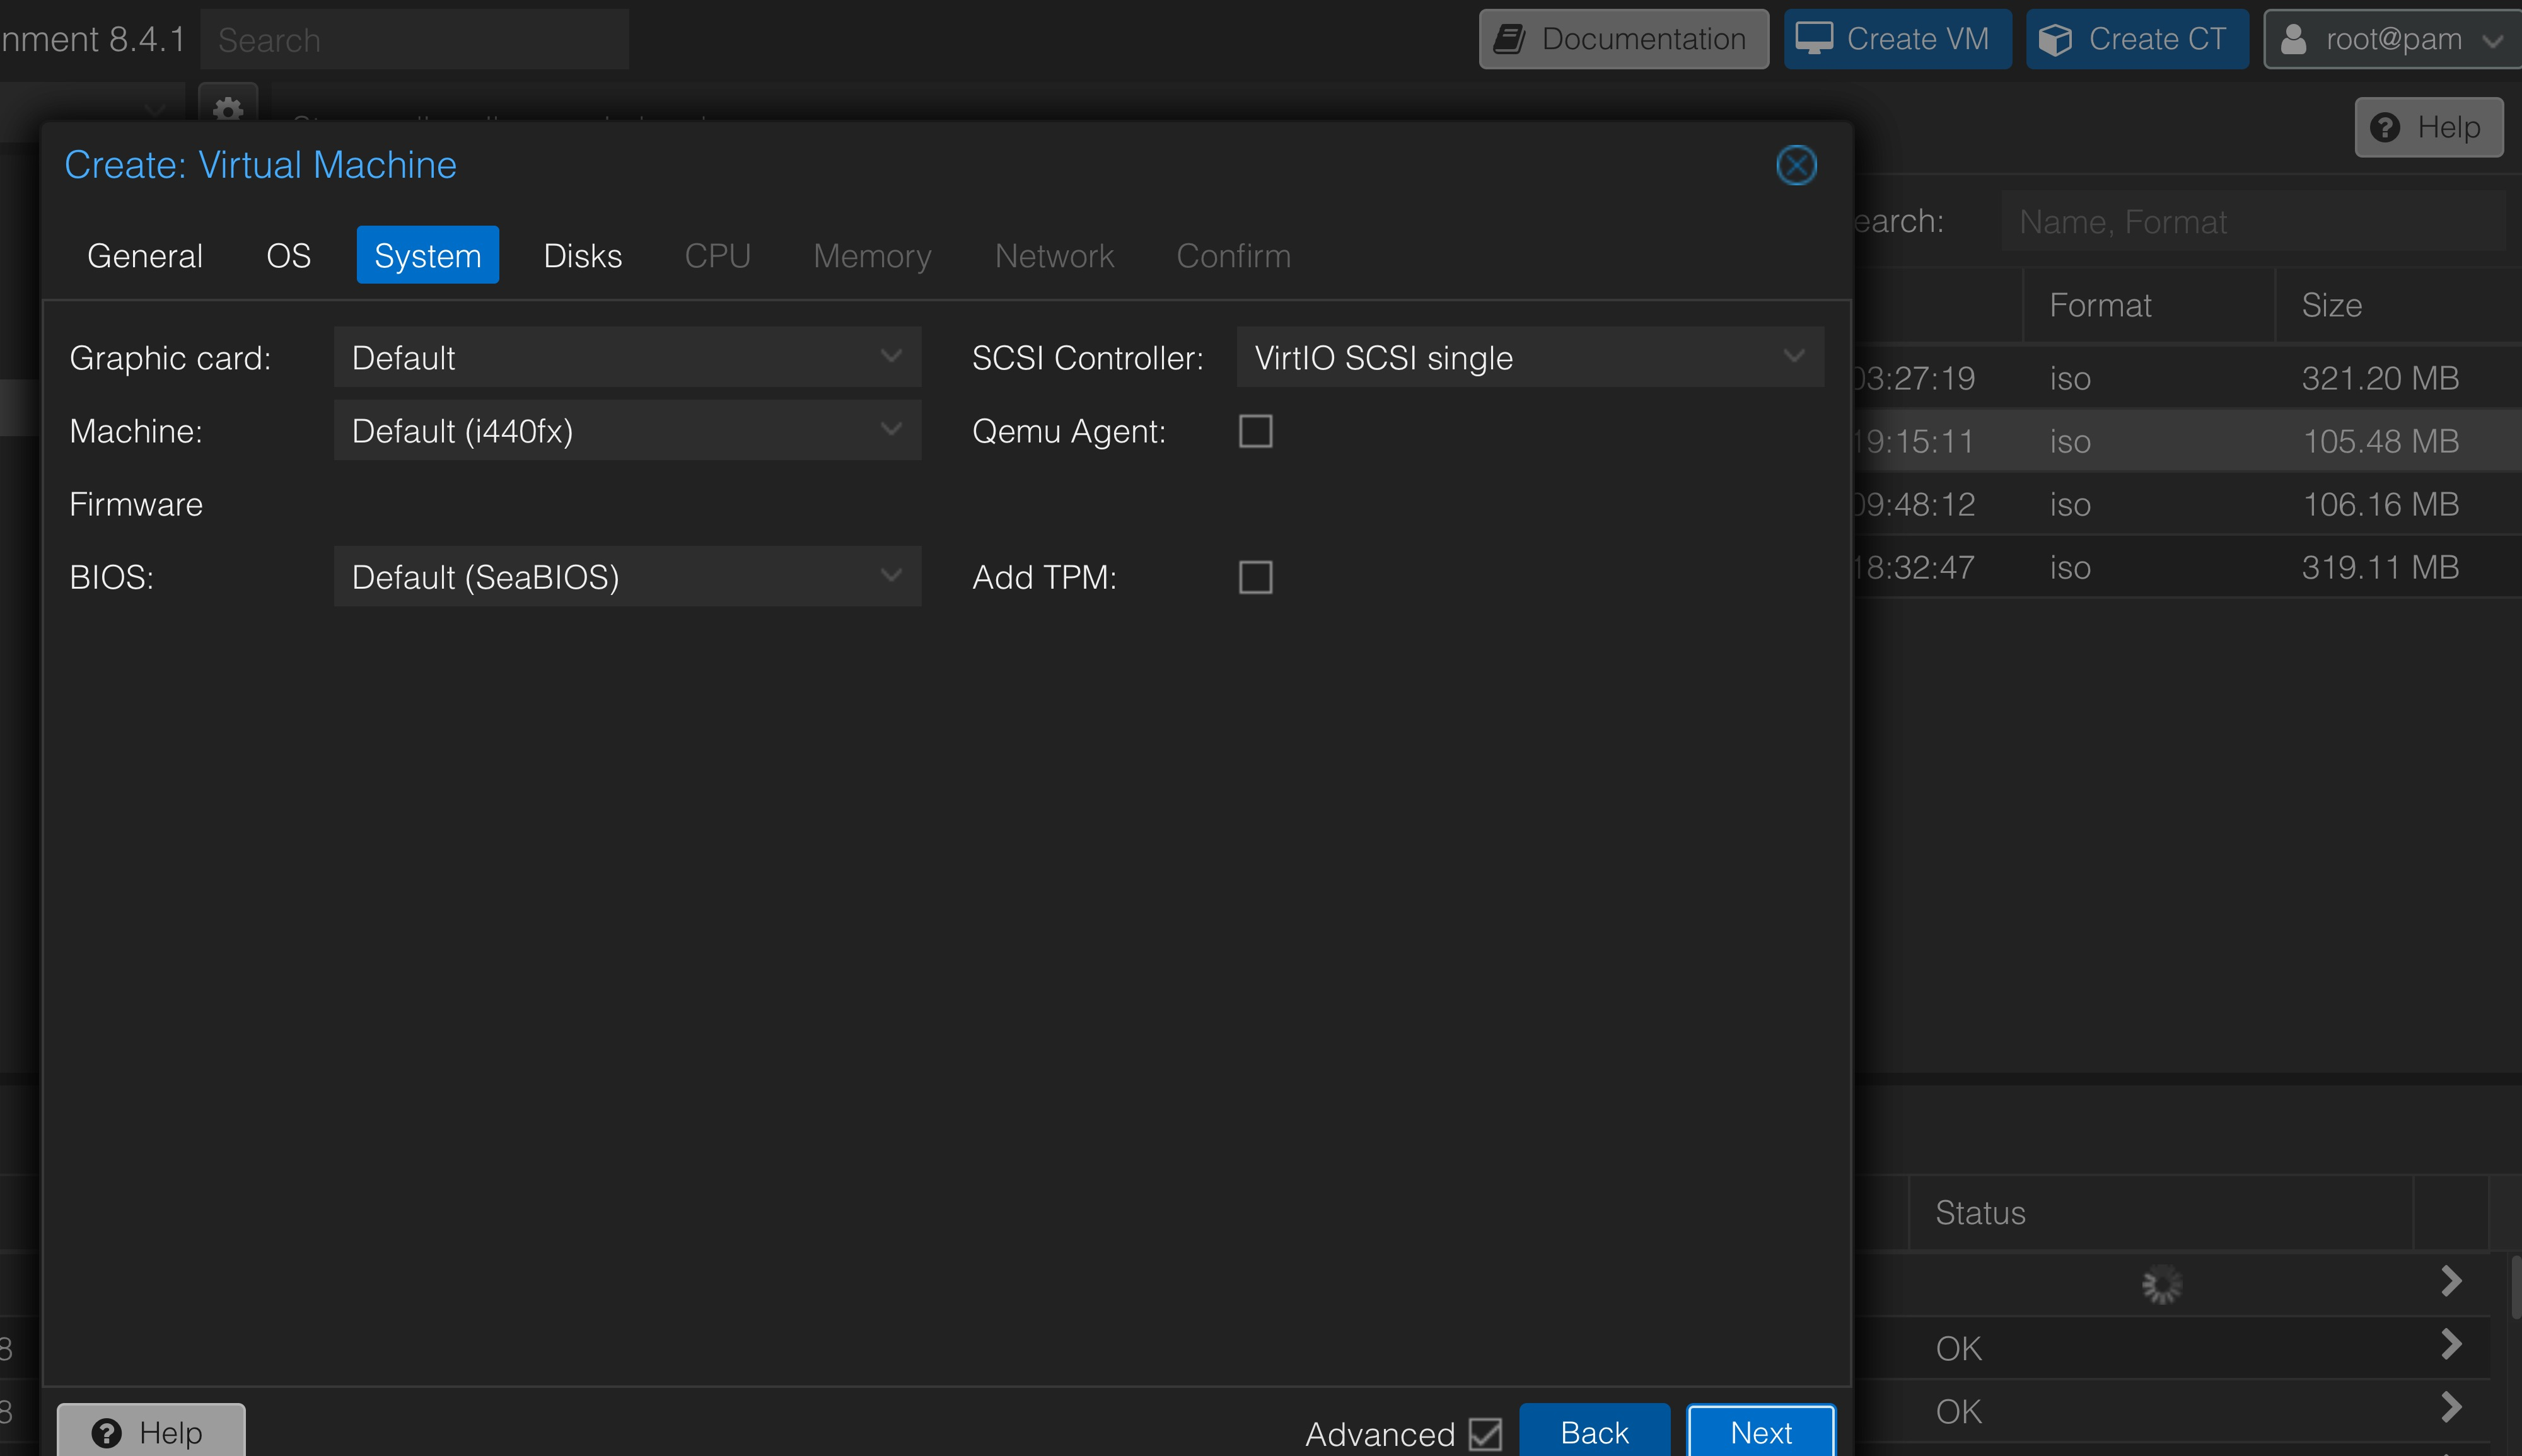
\includegraphics[width=1\textwidth]{figures/talos-install-4.jpg}
    \caption{Instalasi Talos OS 3}
\end{figure}
\begin{figure}[!htbp]
    4. Pada bagian Disk. Cuku merubah bagian Disk size menjadi 100
    \centering
    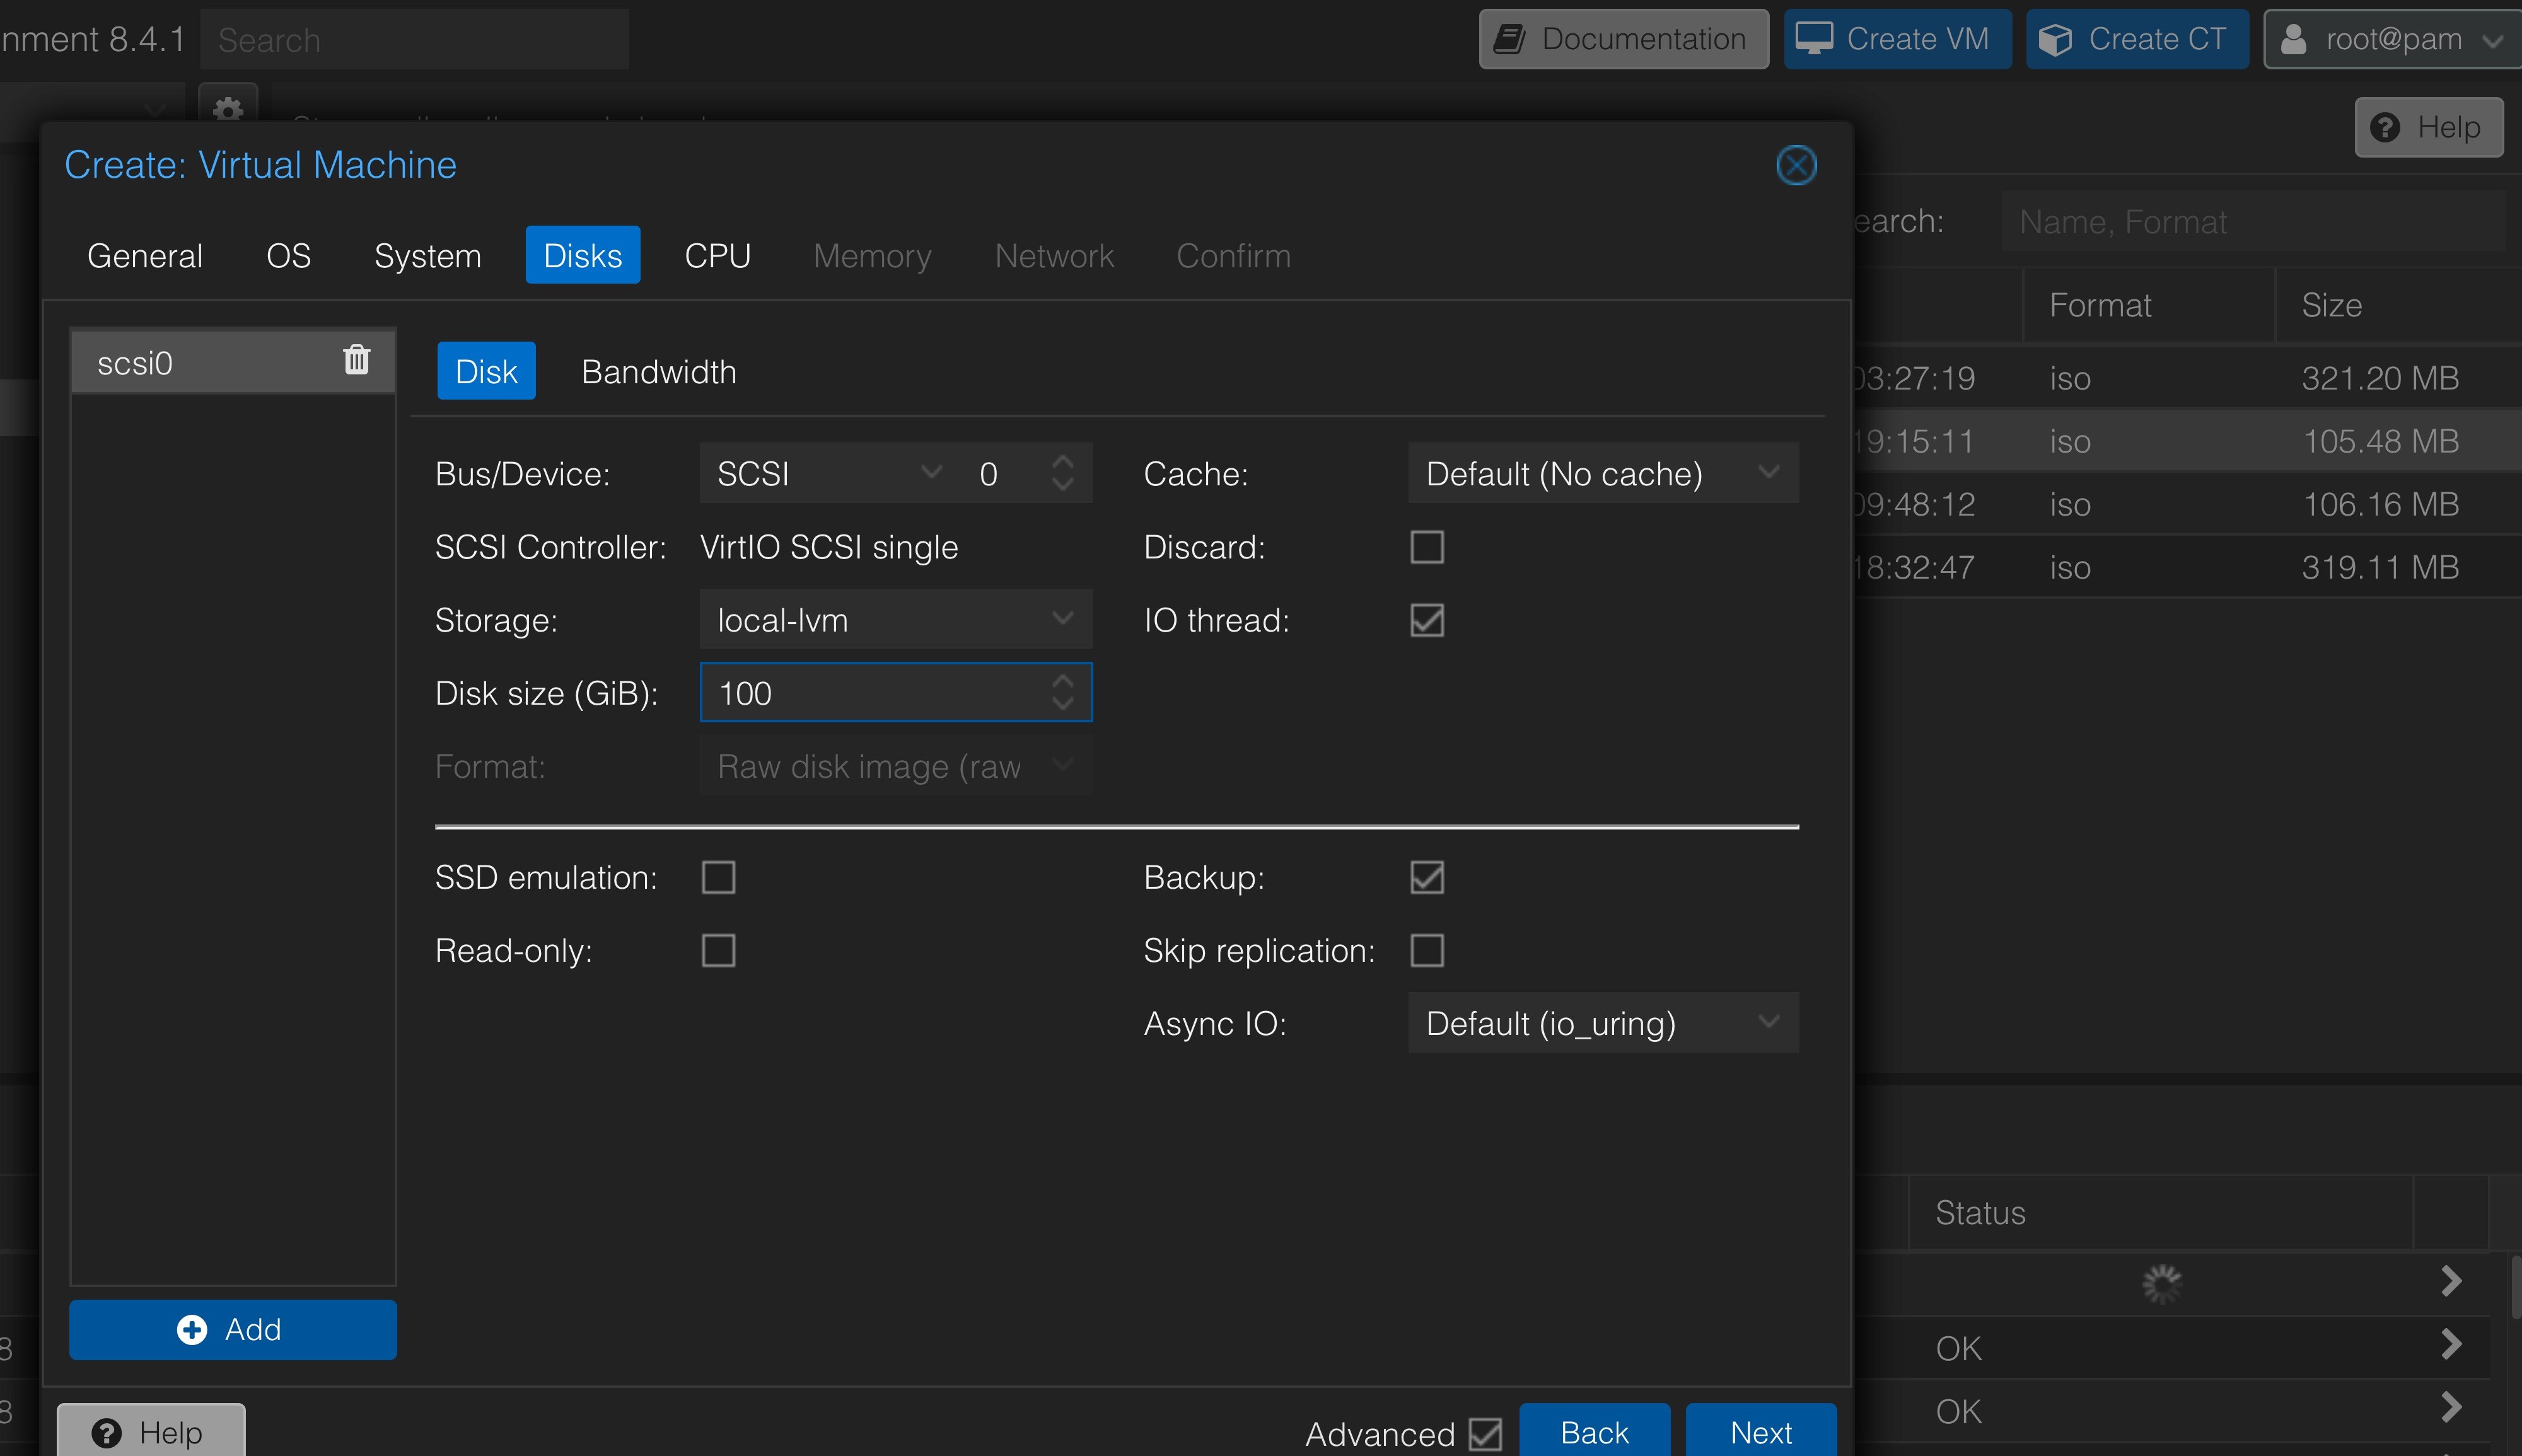
\includegraphics[width=1\textwidth]{figures/talos-install-5.jpg}
    \caption{Instalasi Talos OS 4}
\end{figure}
\begin{figure}[!htbp]
    5. Pada bagian CPU. Cukup merubah cores menjadi 2 atau 4 sesuai spesifikasi mesin yang diinginkan
    \centering
    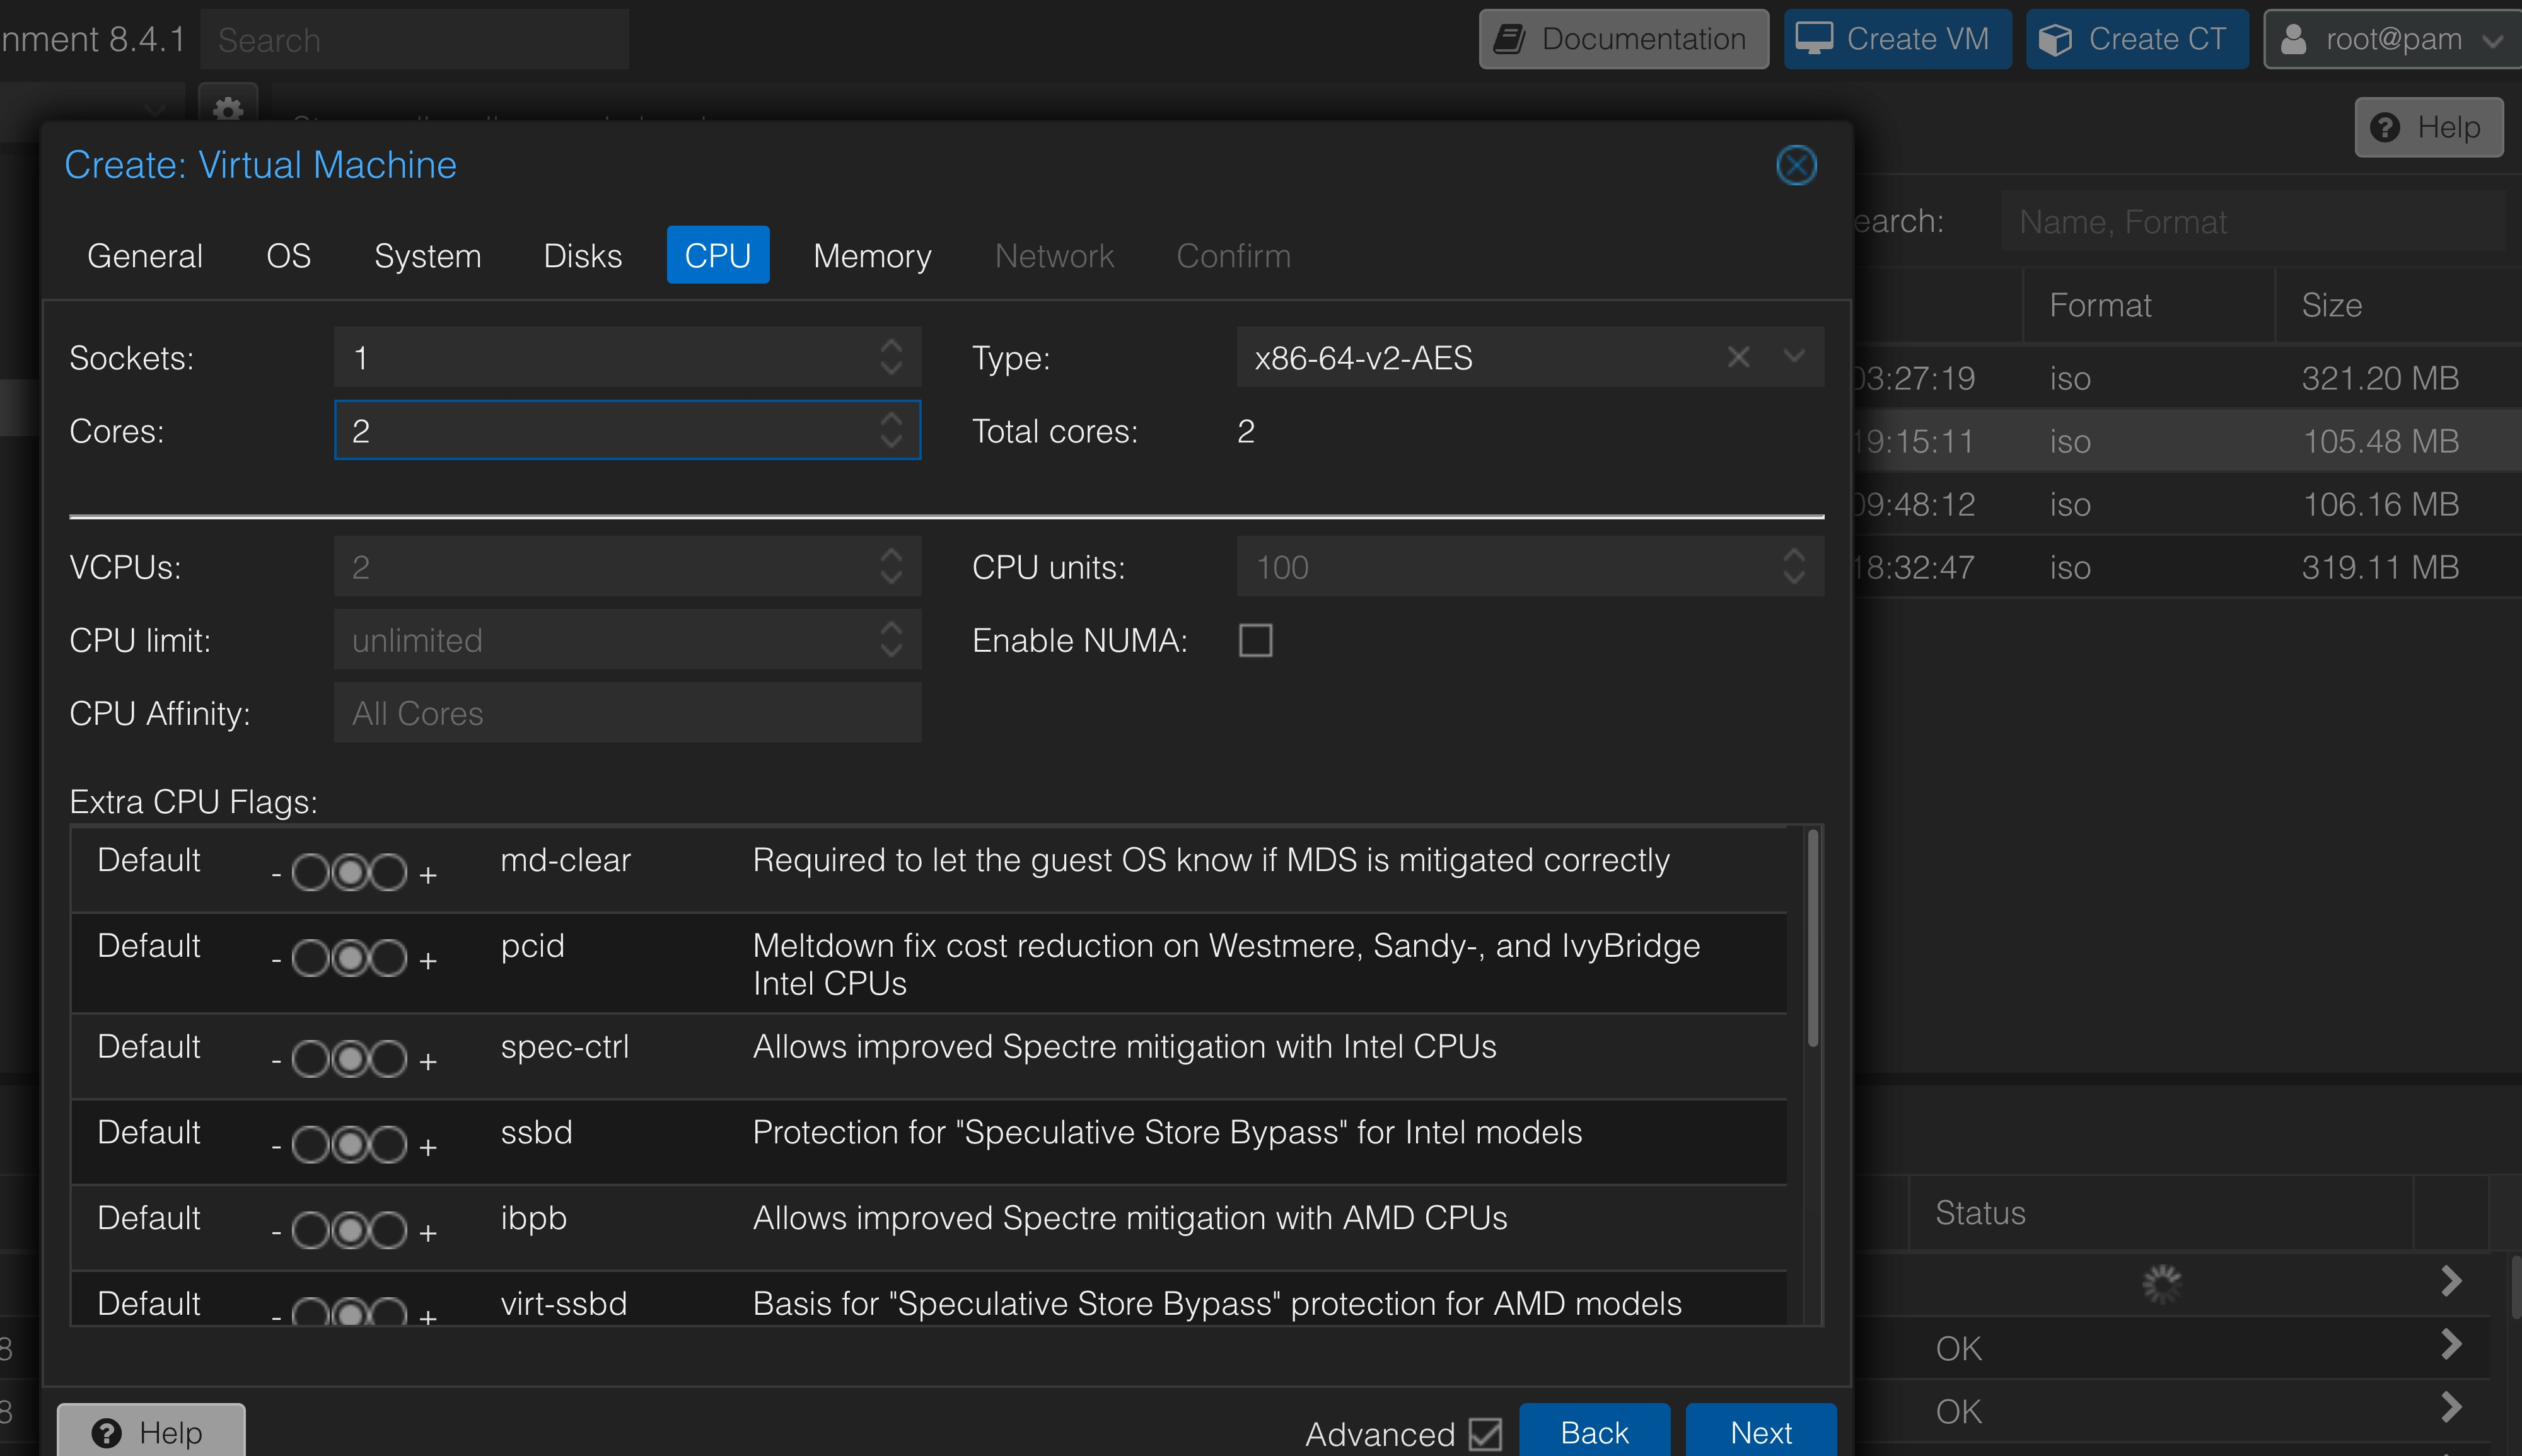
\includegraphics[width=1\textwidth]{figures/talos-install-6.jpg}
    \caption{Instalasi Talos OS 5}
\end{figure}
\begin{figure}[!htbp]
    6. Pada bagian memory. Isikan memory sesuai yang dinginkan dengan minimal 8192 MiB
    \centering
    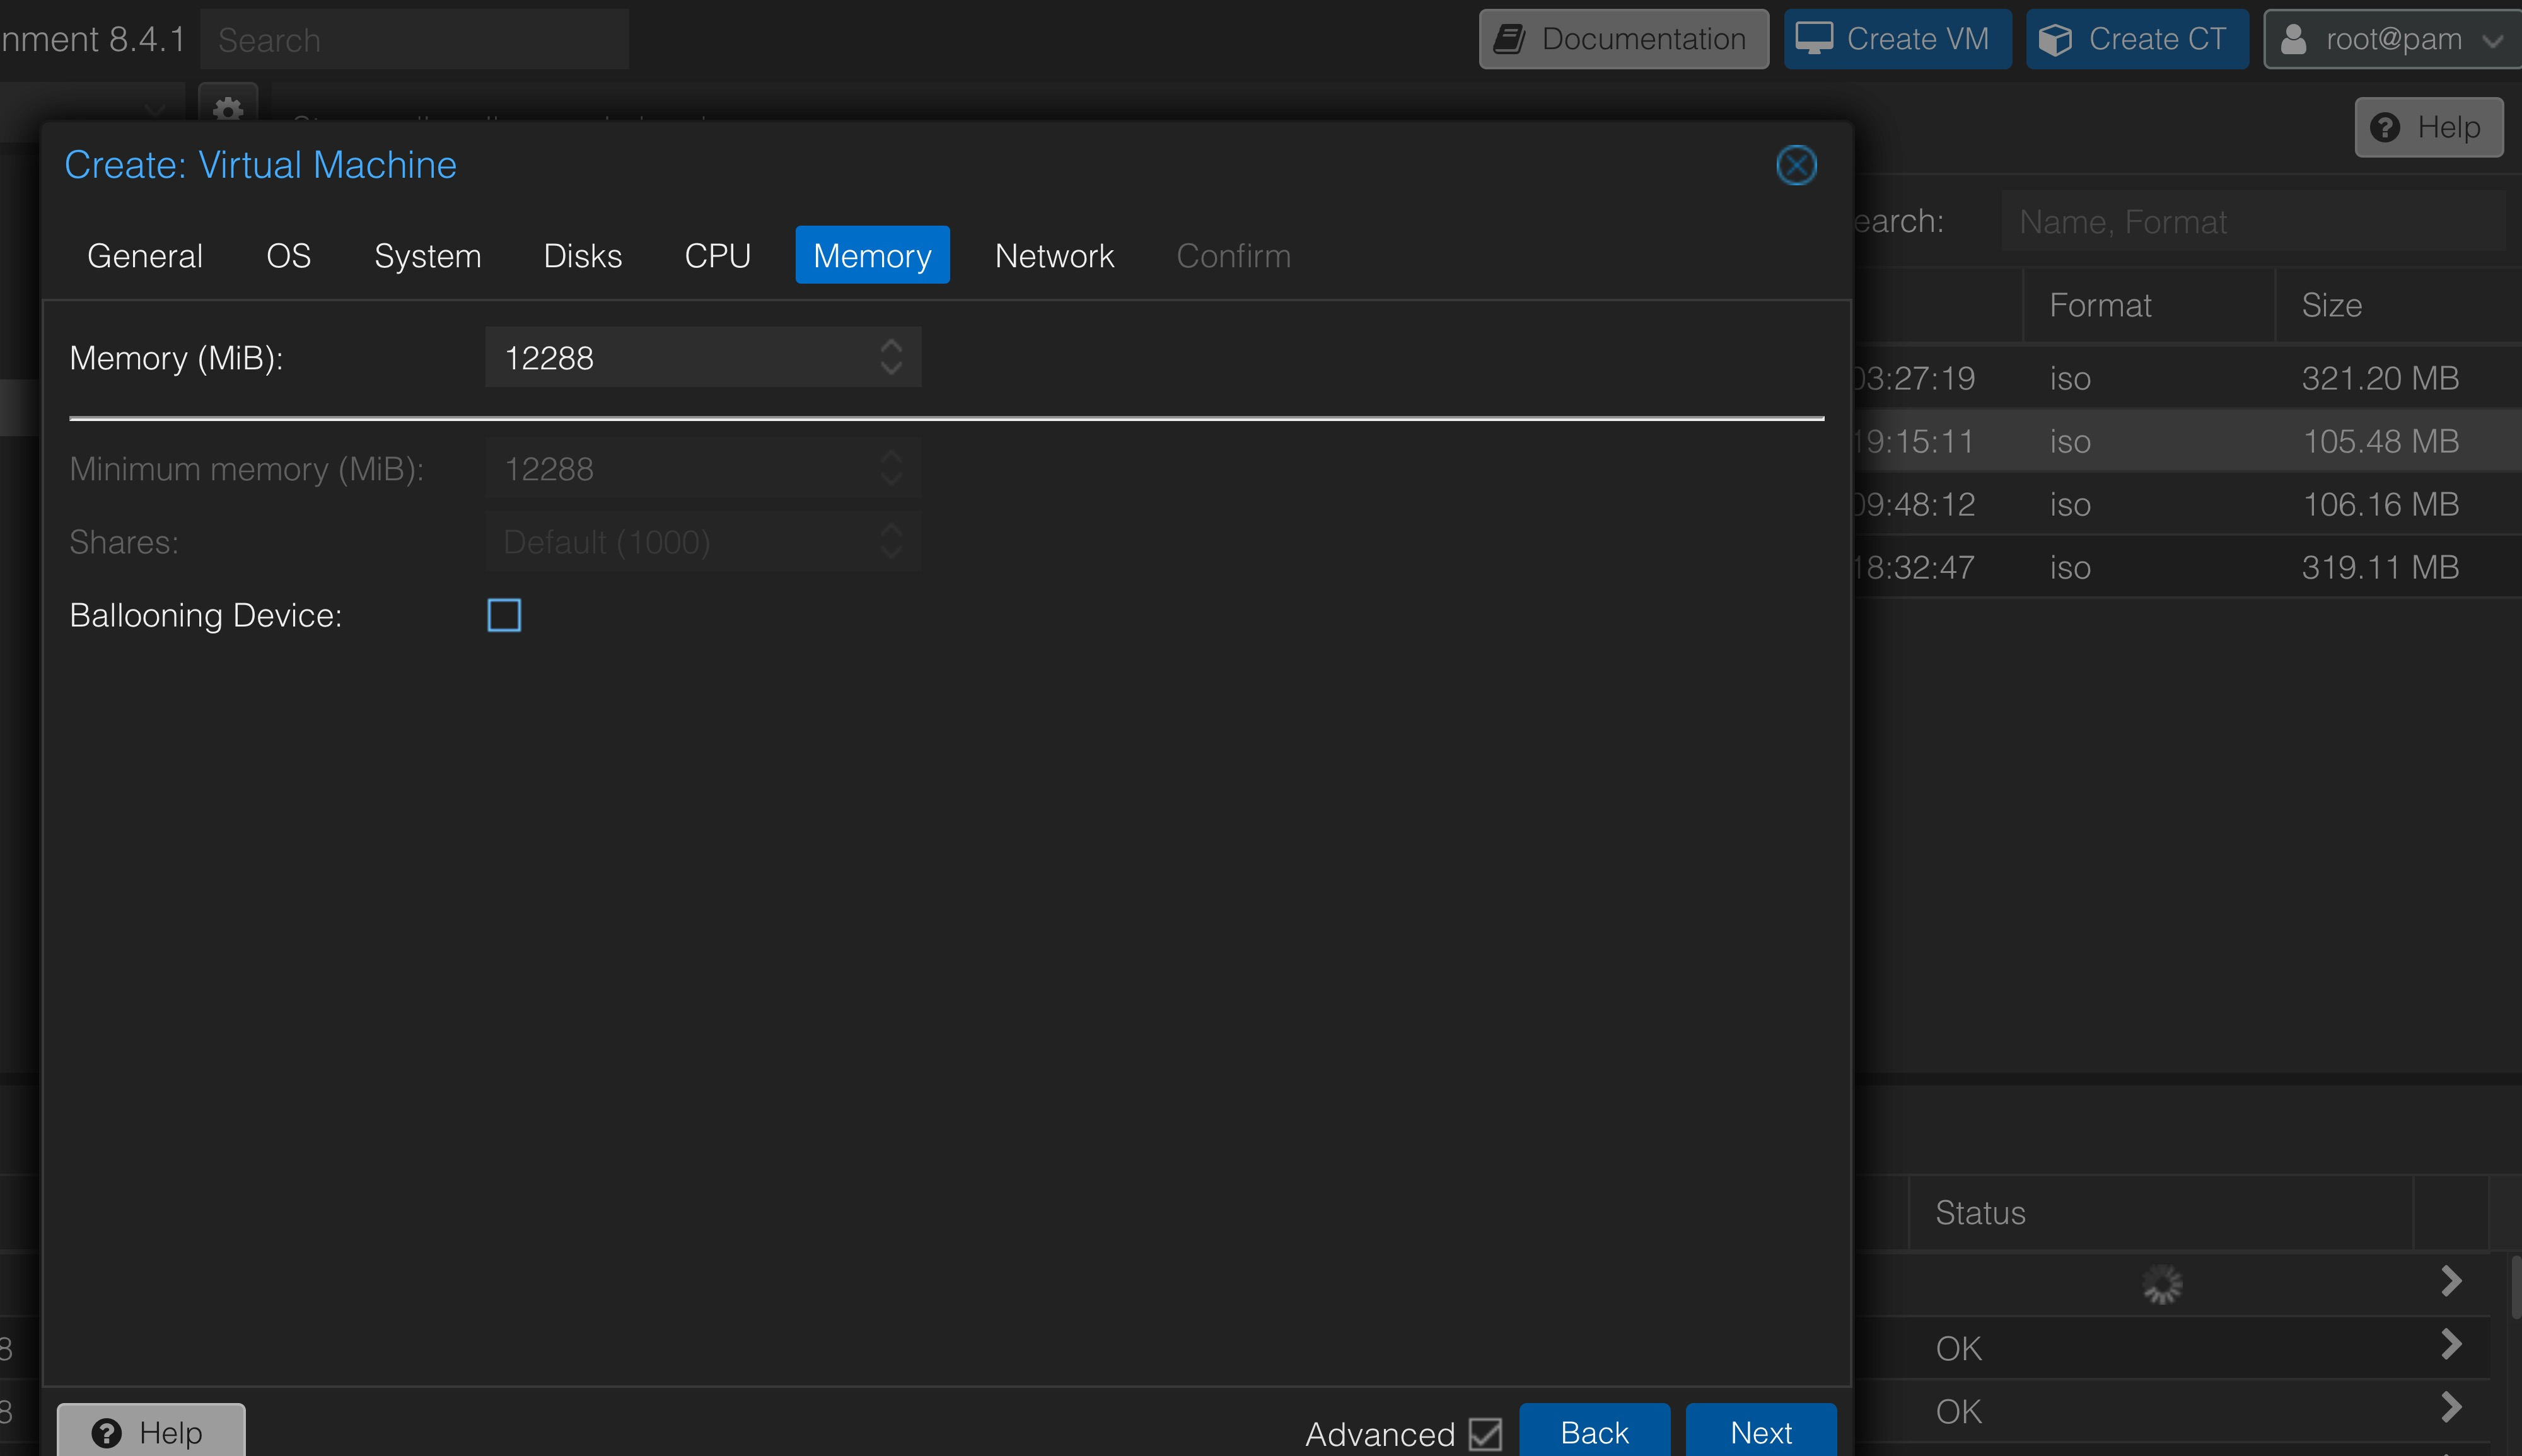
\includegraphics[width=1\textwidth]{figures/talos-install-7.jpg}
    \caption{Instalasi Talos OS 6}
\end{figure}
\begin{figure}[!htbp]
    7. Pada bagian Network. Silahkan klik next
    \centering
    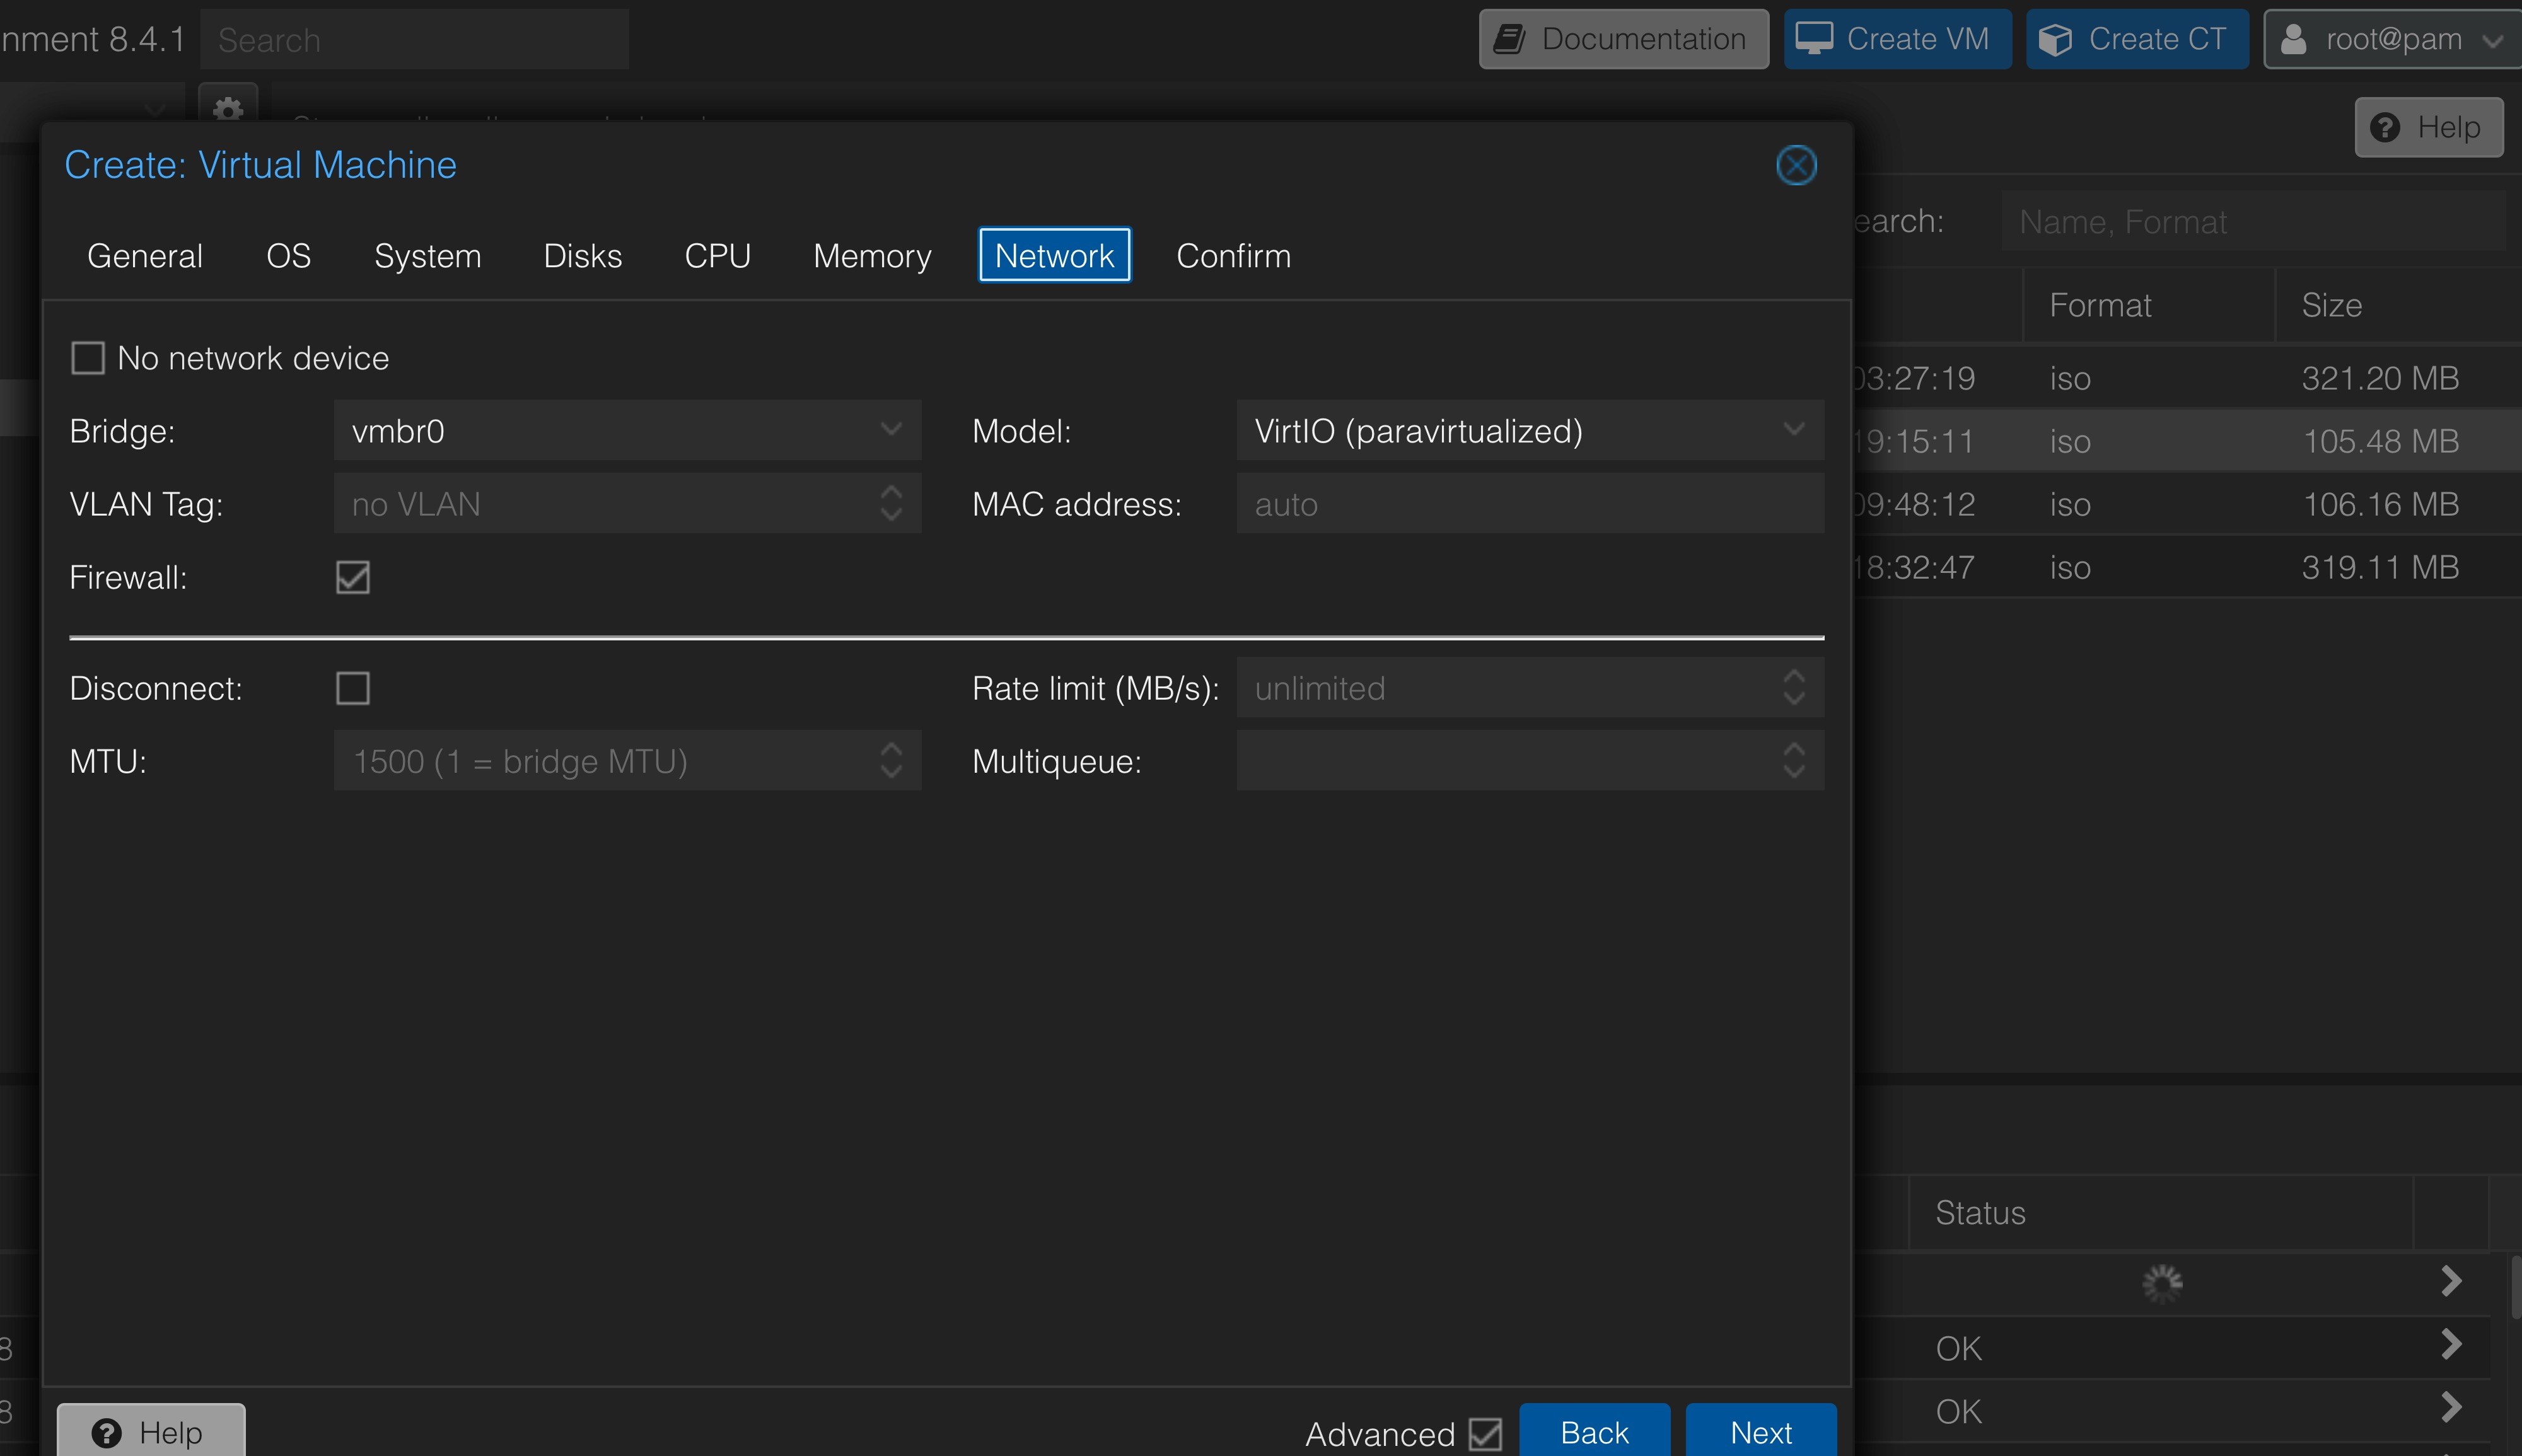
\includegraphics[width=1\textwidth]{figures/talos-install-8.jpg}
    \caption{Instalasi Talos OS 7}
\end{figure}
\begin{figure}[!htbp]
    8. Pada bagian confirm. Centang "Start After Created" lalu Finish
    \centering
    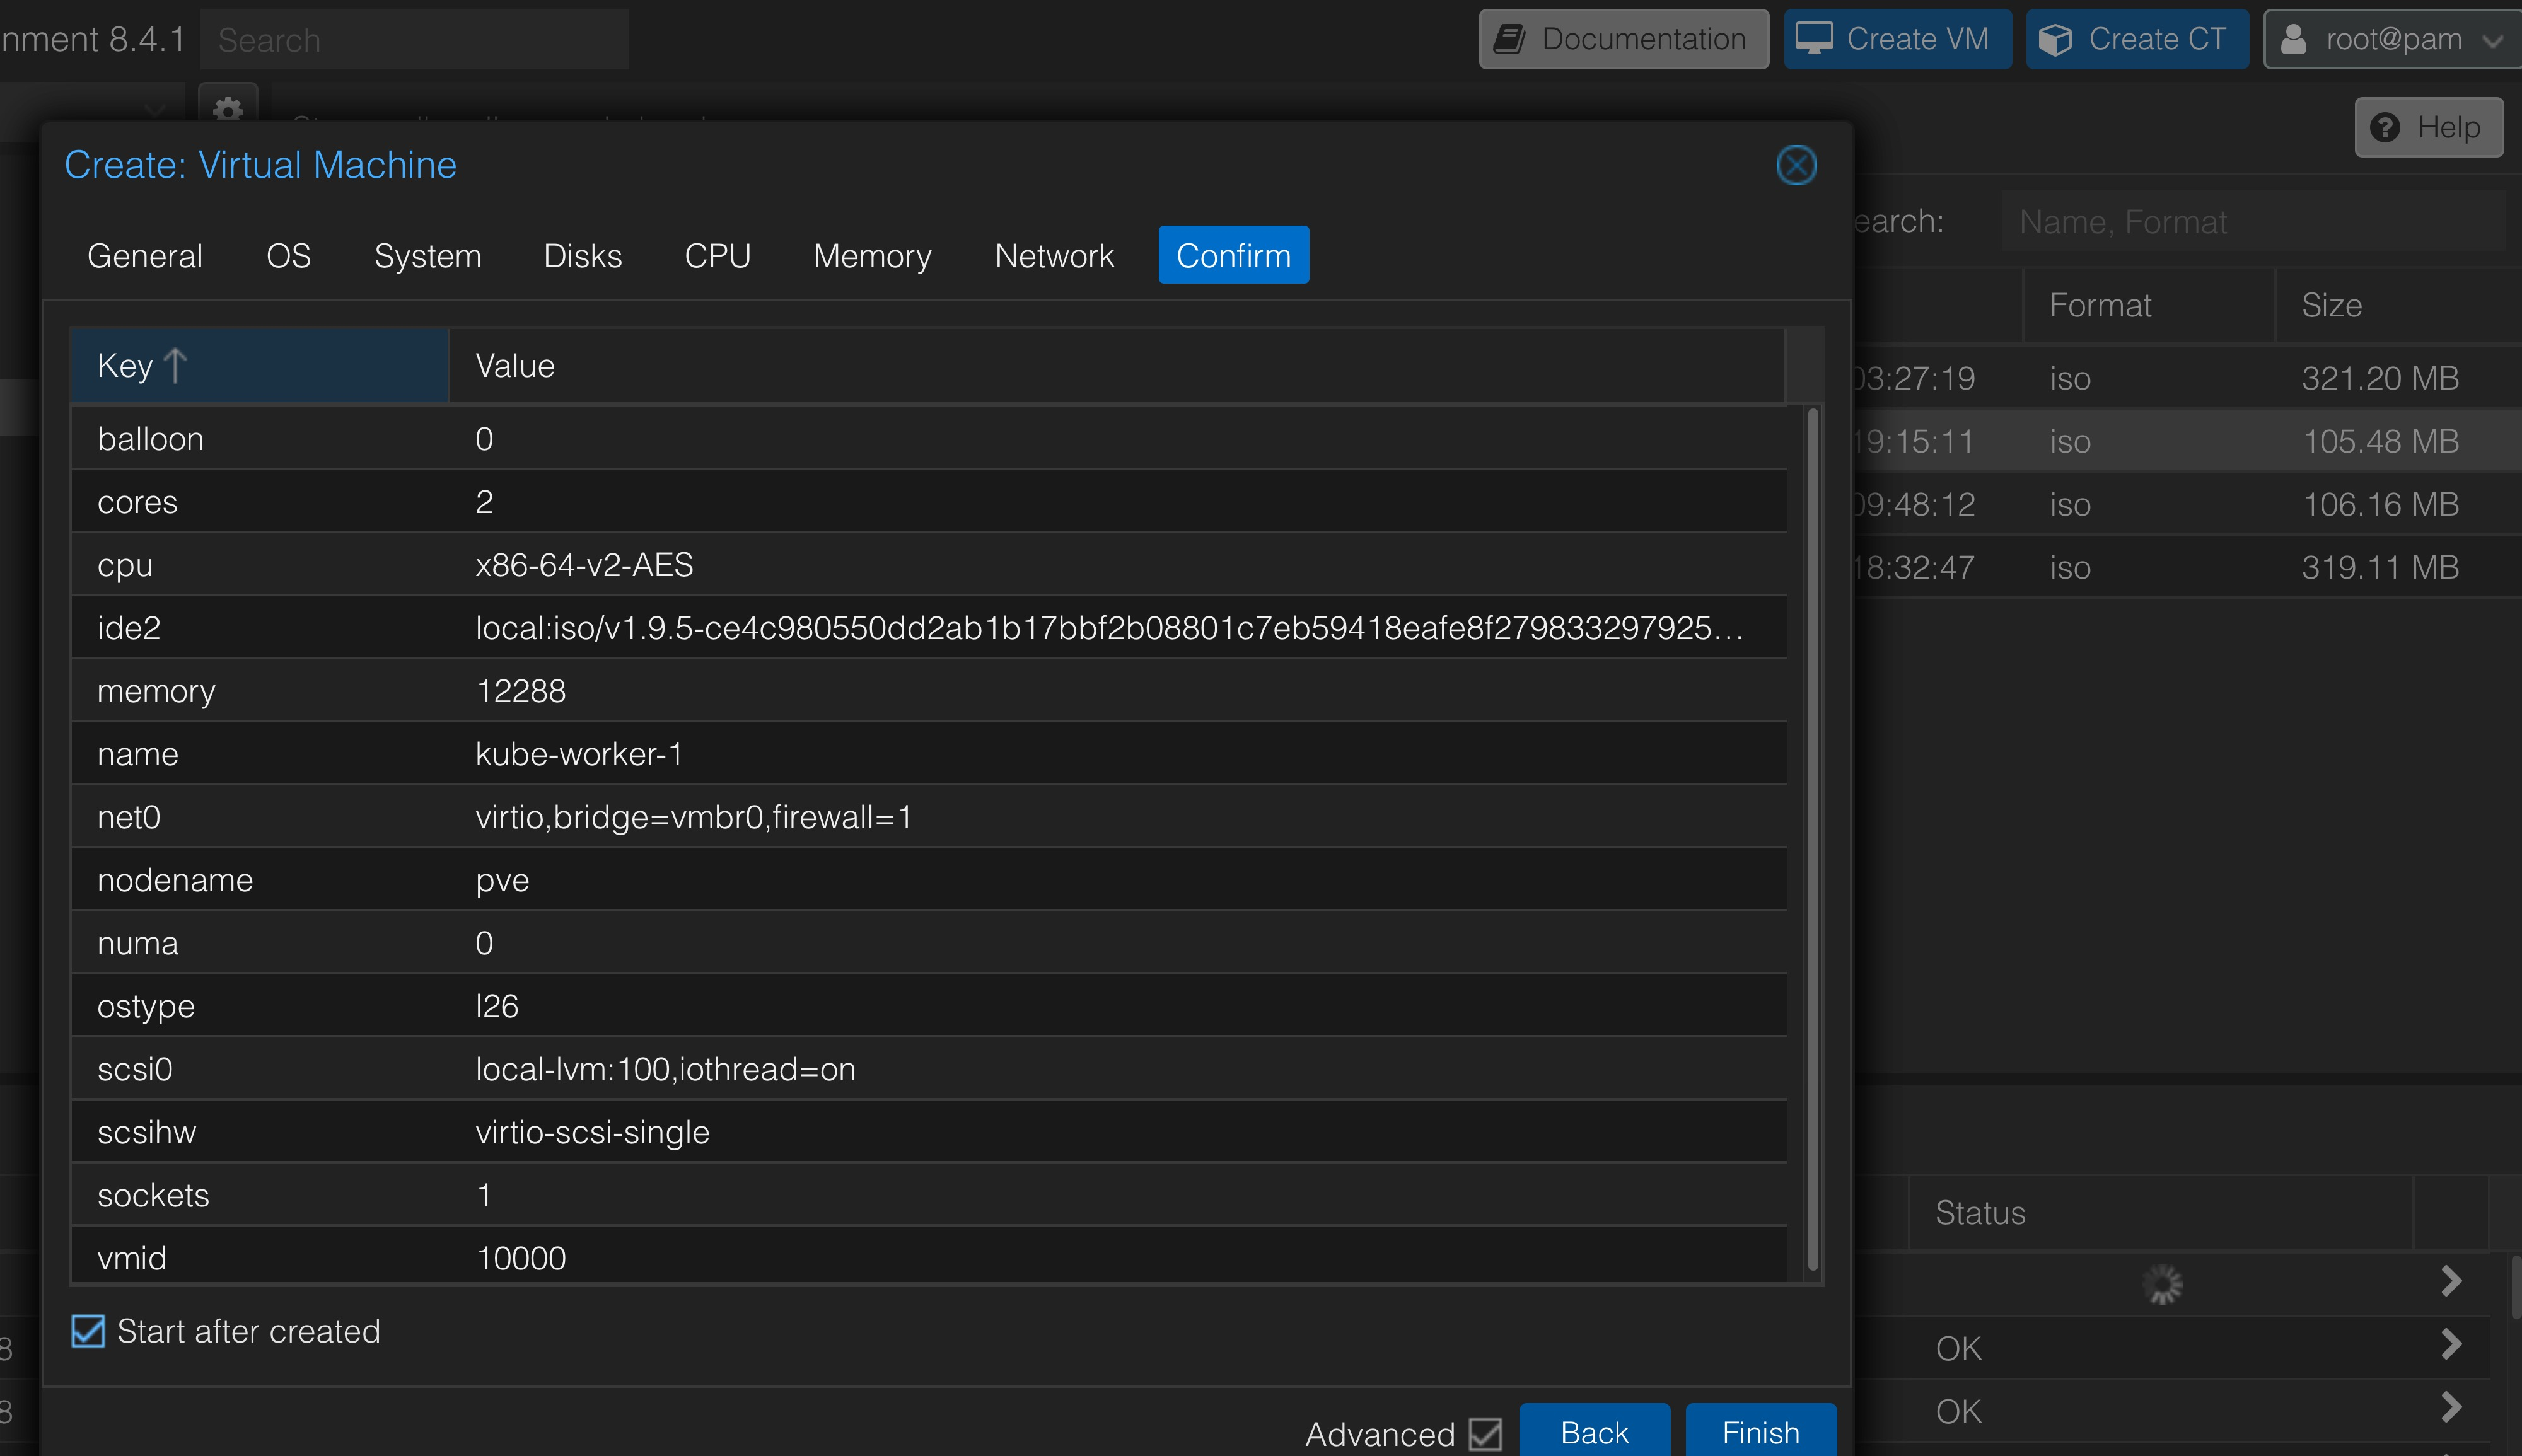
\includegraphics[width=1\textwidth]{figures/talos-install-9.jpg}
    \caption{Instalasi Talos OS 8}
\end{figure}
\begin{figure}[!htbp]
    10. Ketika Talos OS Sudah berjalan terminal Talos OS akan tampak seperti ini
    \centering
    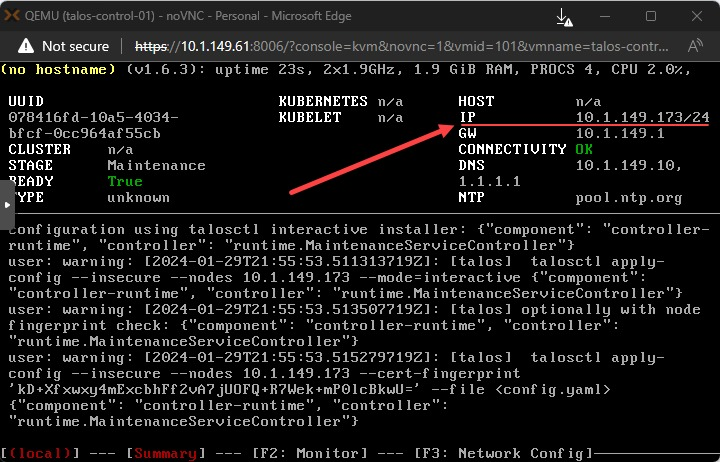
\includegraphics[width=1\textwidth]{figures/talos-install-10.jpg}
    \caption{Instalasi Talos OS 9}
\end{figure}
\newpage

\subsection{Pengkodean Instalasi Kubernetes Script}
Tahap ini adalah tahap untuk instalasi Kubernetes pada Talos OS. Disini peneliti akan menggunakan deklaratif yaml yang akan mengautomatisasi instalasi kubernetes pada Talos OS.
Instalasi Kubernetes pada Talos OS sendiri mengikuti panduan dari pedoman yang terdapat pada website Talos OS \url{https://www.talos.dev/v1.9.5/introduction/getting-started/}

\begin{table}[!htbp]
    \begin{lstlisting}[language=yaml, basicstyle=\footnotesize\ttfamily]
version: '3'
tasks:
  talos:
    desc: Bootstrap the Talos cluster
    dir: '{{.TALOS_DIR}}'
    cmds:
      - '[ -f talsecret.sops.yaml ] || talhelper gensecret | sops --filename-override talos/talsecret.sops.yaml --encrypt /dev/stdin > talsecret.sops.yaml'
      - talhelper genconfig
      - talhelper gencommand apply --extra-flags="--insecure" | bash
      - until talhelper gencommand bootstrap | bash; do sleep 10; done
      - until talhelper gencommand kubeconfig --extra-flags="{{.ROOT_DIR}} --force" | bash; do sleep 10; done
\end{lstlisting}
    \caption{Konfigurasi script instalasi Kubernetes cluster pada Talos OS}
    \label{tab:yaml-code}
\end{table}
\begin{table}[!htbp]
    \begin{lstlisting}[language=yaml, basicstyle=\footnotesize\ttfamily]
clusterName: kubernetes
endpoint: https://192.168.0.250:6443
...
nodes:
  - hostname: "kube-cp-1"
    ipAddress: "192.168.0.200"
    installDisk: "/dev/sda"
    machineSpec:
    controlPlane: true
    networkInterfaces:
      - deviceSelector:
          hardwareAddr: "de:ad:be:ef:00:01"
        addresses:
          - "192.168.0.200/24"
        routes:
          - network: "0.0.0.0/0"
            gateway: "192.168.0.1"
        mtu: 1500
        vip:
          ip: "192.168.0.250"
  - hostname: "kube-worker-1"
    ipAddress: "192.168.0.201"
    installDisk: "/dev/sda"
    machineSpec:
    controlPlane: false
    networkInterfaces:
      - deviceSelector:
          hardwareAddr: "de:ad:be:ef:00:02"
        dhcp: false
        addresses:
          - "192.168.0.201/24"
        routes:
          - network: "0.0.0.0/0"
            gateway: "192.168.0.1"
        mtu: 1500
\end{lstlisting}
    \caption{Konfigurasi script instalasi Kubernetes cluster pada Talos OS}
    \label{tab:yaml-code-2}
\end{table}
\newpage
Setelah dilakukan instalasi Kubernetes cluster pada Talos OS tampilan terminal akan menampilkan nama cluster
dan juga sudah tidak menampilan status Stage: Maintenance seperti Gambar 4.16.
\begin{figure}[!ht]
    \centering
    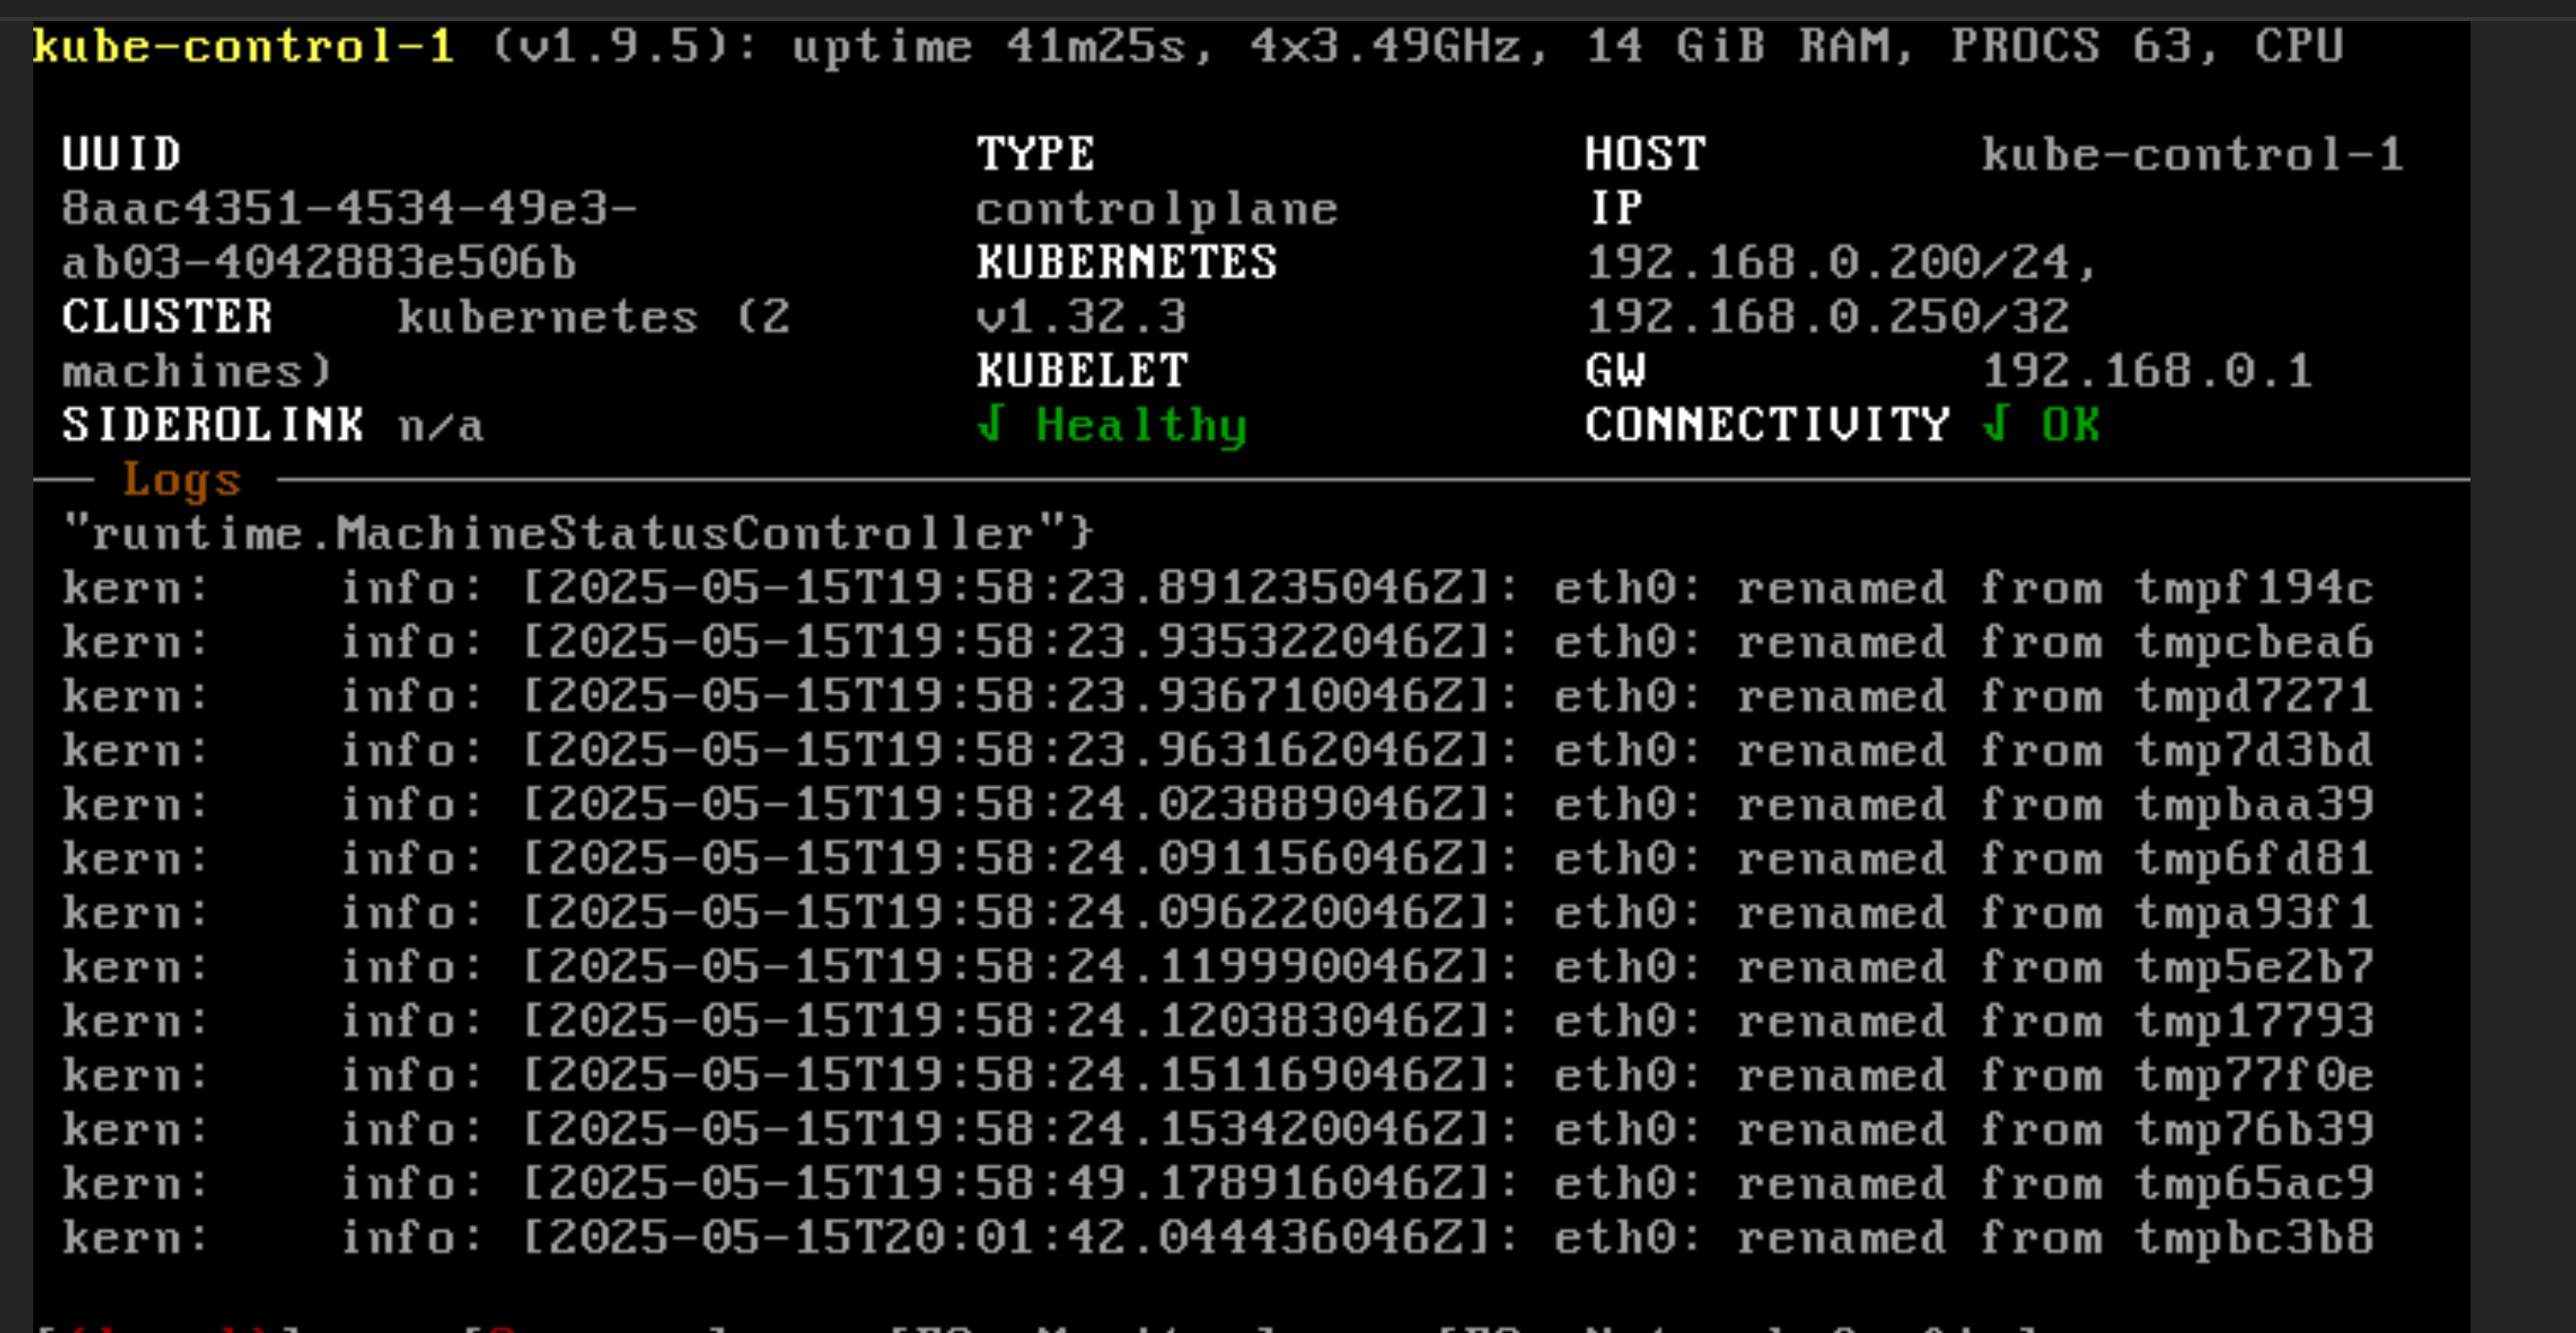
\includegraphics[width=1\textwidth]{figures/talos-install-11.jpg}
    \caption{Tampilan Talos OS setelah instalasi kubernetes cluster}
\end{figure}
\newpage
Setelah instalasi kubernetes pada Talos OS dilakukan maka kita dapat mengakses kubernetes cluster tersebut menggunakan cli kubectl.
Sebagai contoh saya mempunyai aplikasi yang menampilkan informasi header pada browser pada \url{echo.zeinfahrozi.my.id}
\begin{figure}[!ht]
    \centering
    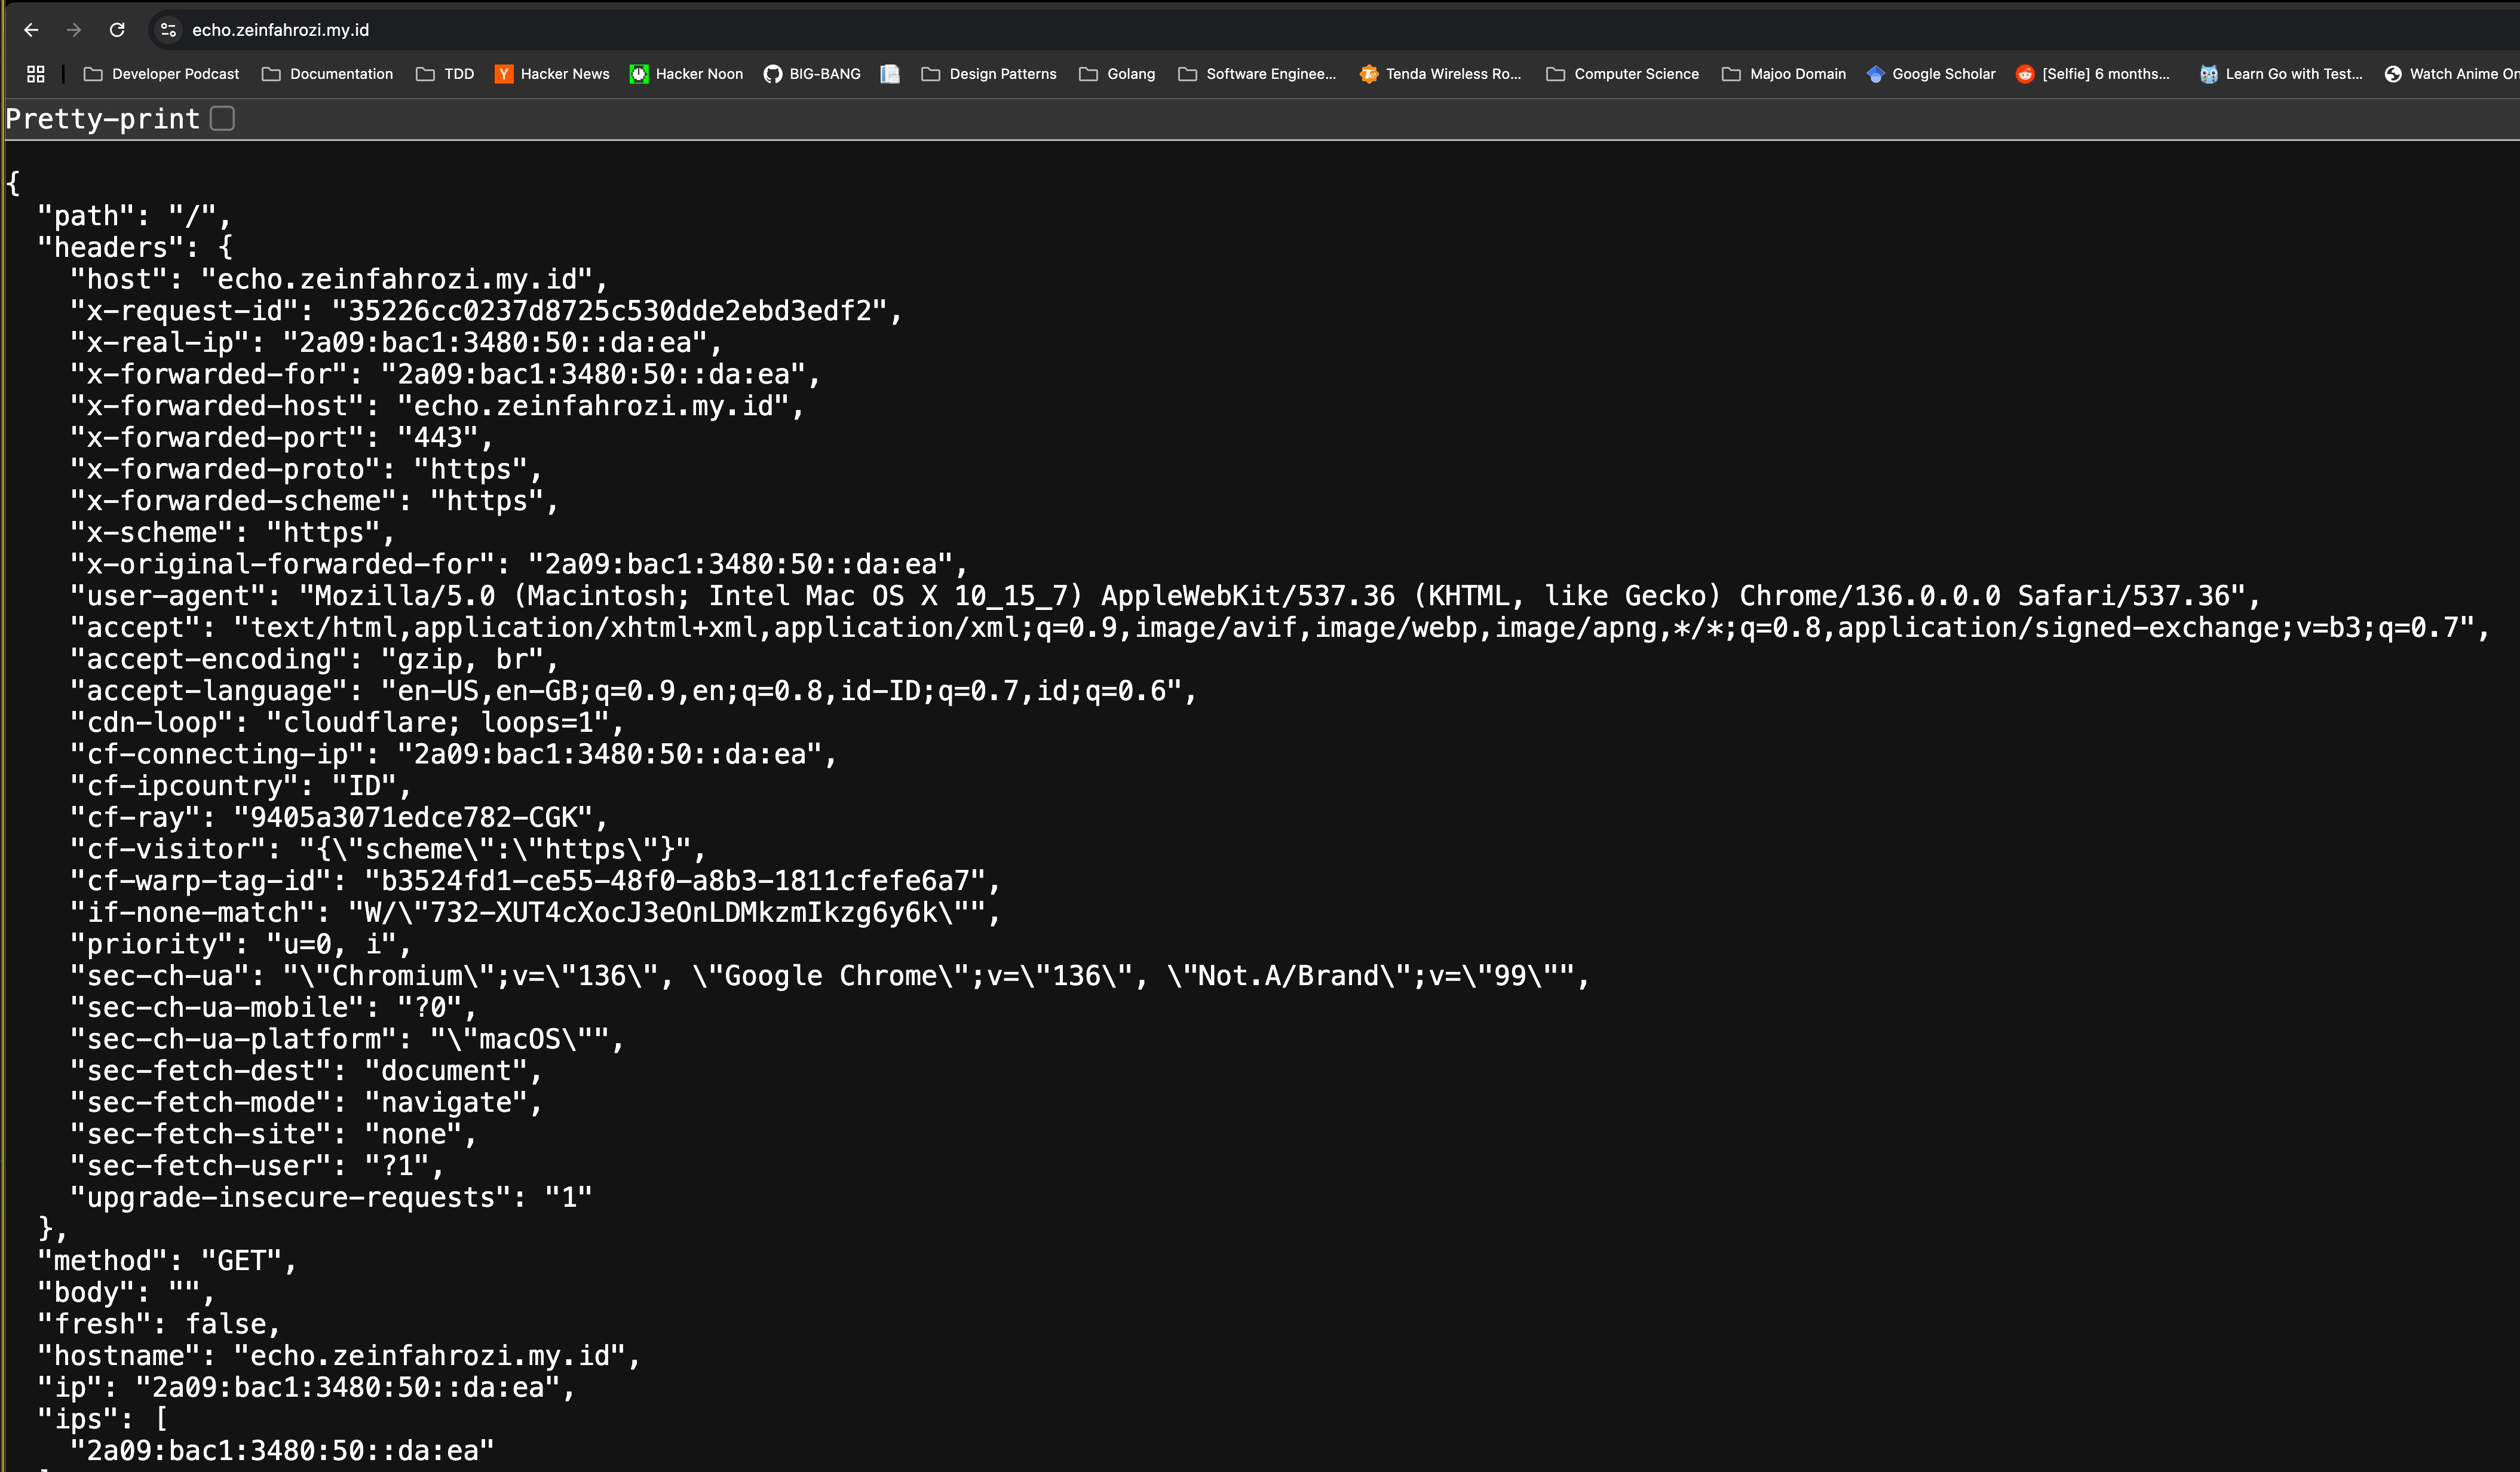
\includegraphics[width=1\textwidth]{figures/echo-web.jpg}
    \caption{Tampilan echo.zeinfahrozi.my.id pada browser}
\end{figure}
\section{Implementasi ArgoCD pada cluster kubernetes}
Tahap ini merupakan instalasi instance ArgoCD itu sendiri pada kubernetes cluster yang sudah dibuat sebelumnya. ArgoCD dipasang menggunakan Helm chart dengan konfigurasi kustom yang disesuaikan dengan kebutuhan lingkungan produksi.

Berikut adalah contoh perintah untuk menginstal ArgoCD menggunakan Helm:

\begin{lstlisting}[language=bash, basicstyle=\footnotesize\ttfamily]
# Menambahkan repo ArgoCD
helm repo add argo https://argoproj.github.io/argo-helm
helm repo update

# Membuat namespace untuk ArgoCD
kubectl create namespace argocd

# Menginstal ArgoCD dengan Helm
helm upgrade --install argocd argo/argo-cd \
  --namespace argocd \
  --values values.sops.yaml \
  --wait
\end{lstlisting}

\subsection{Instalasi ArgoCD}
ArgoCD diinstal menggunakan Helm dengan nilai-nilai kustom yang didefinisikan dalam file konfigurasi. Berikut adalah contoh konfigurasi \texttt{values.sops.yaml} yang digunakan:

\begin{lstlisting}[language=yaml, basicstyle=\footnotesize\ttfamily]
# values.sops.yaml
crds:
  install: true

global:
  domain: argo.zeinfahrozi.my.id

configs:
  params:
    server.insecure: true
  cm:
    statusbadge.enabled: true
    kustomize.buildOptions: --enable-alpha-plugins --enable-exec
    helm.valuesFileSchemes: >-
      secrets+gpg-import,secrets+gpg-import-kubernetes,
      secrets+age-import,secrets+age-import-kubernetes,
      secrets,secrets+literal,https
    resource.exclusions: |
      - apiGroups:
          - cilium.io
        kinds:
          - CiliumIdentity
        clusters:
          - "*"
\end{lstlisting}

Beberapa konfigurasi penting yang diterapkan:

\begin{itemize}
    \item ArgoCD diakses melalui domain \texttt{argo.zeinfahrozi.my.id}
    \item Mode \texttt{insecure} diaktifkan untuk pengembangan
    \item Fitur status badge diaktifkan untuk memantau status aplikasi
    \item Dukungan untuk multiple value files dengan skema yang berbeda
    \item Eksklusi sumber daya tertentu seperti CiliumIdentity dari manajemen ArgoCD
\end{itemize}

\subsection{Konfigurasi High Availability}
Untuk memastikan ketersediaan tinggi, komponen-komponen kritis ArgoCD dikonfigurasi dengan multiple replica:

\begin{itemize}
    \item ArgoCD Server: 2 replica
    \item ArgoCD Controller: 2 replica
    \item Dex Server: 2 replica
\end{itemize}

\subsection{Integrasi dengan Monitoring}
ArgoCD terintegrasi dengan stack monitoring yang sudah ada di cluster melalui ServiceMonitor untuk memantau metrik dari komponen-komponennya:

\begin{itemize}
    \item ArgoCD Server metrics
    \item ArgoCD Controller metrics
    \item Dex Server metrics
    \item Redis metrics
\end{itemize}

\subsection{Manajemen Aplikasi}
Setelah ArgoCD terinstal, aplikasi-aplikasi dapat dikelola menggunakan GitOps. Setiap aplikasi didefinisikan sebagai kustom resource Kubernetes yang mereferensikan repositori Git yang berisi manifest Kubernetes. ArgoCD akan secara otomatis melakukan sinkronisasi antara status yang diinginkan (yang didefinisikan di Git) dengan status aktual di cluster.

\subsection{Keamanan}
Beberapa aspek keamanan yang diterapkan pada instalasi ArgoCD ini antara lain:

\begin{itemize}
    \item Penggunaan HTTPS untuk akses web UI
    \item Integrasi dengan Dex untuk autentikasi
    \item Pembatasan akses berbasis peran (RBAC)
    \item Penyimpanan rahasia yang aman menggunakan SOPS
\end{itemize}

Dengan konfigurasi ini, ArgoCD siap digunakan untuk mengelola aplikasi secara deklaratif menggunakan prinsip GitOps, di mana semua perubahan konfigurasi dilakukan melalui pull request dan version control system.

\section{Implementasi Cloudflare Tunnel}
Cloudflare Tunnel digunakan untuk mengekspos layanan dalam cluster ke internet dengan aman tanpa perlu membuka port firewall. Berikut adalah langkah-langkah implementasinya:

1. **Persiapan**
- Memiliki akun Cloudflare
- Mendaftarkan domain yang akan digunakan
- Mengatur DNS di Cloudflare

2. **Instalasi Cloudflare Tunnel**
Cloudflare Tunnel diinstal menggunakan ArgoCD dengan konfigurasi sebagai berikut:

\begin{lstlisting}[language=yaml, basicstyle=\footnotesize\ttfamily]
# cloudflared.yaml
apiVersion: argoproj.io/v1alpha1
kind: Application
metadata:
     name: cloudflared
     namespace: argo-system
   spec:
     project: kubernetes
     sources:
       - repoURL: "https://github.com/mozarik/zein-home-lab.git"
         path: kubernetes/apps/network/cloudflared
         targetRevision: main
     destination:
       name: in-cluster
       namespace: network
     syncPolicy:
       automated:
         prune: true
         selfHeal: true
\end{lstlisting}

3. **Konfigurasi Tunnel**
Setelah terinstal, Cloudflare Tunnel perlu dikonfigurasi untuk meneruskan lalu lintas ke layanan dalam cluster. Berikut contoh konfigurasi untuk mengekspos ArgoCD:

\begin{lstlisting}[language=yaml, basicstyle=\footnotesize\ttfamily]
   # config.yaml
   tunnel: <tunnel-id>
   credentials-file: /etc/cloudflared/credentials.json
   ingress:
     - hostname: argo.zeinfahrozi.my.id
       service: http://argocd-server.argocd.svc.cluster.local:80
     - service: http_status:404
   \end{lstlisting}

\subsection{Konfigurasi Git Repository}
Git repository digunakan sebagai sumber kebenaran (source of truth) untuk konfigurasi infrastruktur. Repository yang digunakan adalah \url{https://github.com/mozarik/zein-home-lab} dengan struktur sebagai berikut:


Alur kerja GitOps yang diterapkan:
1. Perubahan konfigurasi dilakukan melalui pull request
2. Setelah pull request disetujui dan digabungkan ke branch main
3. ArgoCD secara otomatis mendeteksi perubahan dan melakukan sinkronisasi dengan cluster

\subsection{Integrasi dengan GitHub Actions}
Untuk memastikan kualitas kode dan keamanan, diterapkan GitHub Actions workflow yang akan:
1. Melakukan linting pada file konfigurasi Kubernetes
2. Melakukan validasi dengan kubeval
3. Melakukan pengecekan keamanan dengan kubesec

Contoh workflow GitHub Actions:

\begin{lstlisting}[language=yaml, basicstyle=\footnotesize\ttfamily]
name: Lint and Validate

on:
  push:
    branches: [ main ]
  pull_request:
    branches: [ main ]

jobs:
  lint-validate:
    runs-on: ubuntu-latest
    steps:
      - uses: actions/checkout@v3
      
      - name: Lint Kubernetes files
        uses: azure/k8s-manifests-base@v1
        with:
          action: lint
          files: '**/*.yaml'

      - name: Validate Kubernetes files
        uses: azure/k8s-manifests-base@v1
        with:
          action: validate
          files: '**/*.yaml'
\end{lstlisting}

Dengan konfigurasi ini, seluruh perubahan infrastruktur dapat dilacak melalui riwayat Git, dan proses deployment menjadi lebih terotomatisasi dan konsisten.

\section{Testing}
Setelah menyelesaikan tahap instalasi dan konfigurasi infrastruktur, langkah selanjutnya adalah melakukan pengujian untuk memastikan seluruh komponen berfungsi seperti yang diharapkan. Pengujian ini mencakup beberapa aspek penting termasuk fungsionalitas Kubernetes cluster, integrasi ArgoCD, serta alur kerja GitOps yang telah diterapkan. Melalui pengujian menyeluruh ini, diharapkan dapat dievaluasi sejauh mana solusi yang dibangun mampu memenuhi kebutuhan pengembangan dan operasional aplikasi secara efisien.

\subsection{Pengujian (Testing)}\label{sec:bab4_pengujian}
Pengujian black-box testing yang dilakukan terhadap sistem pada tahap ini menggunakan metode validasi (validation). Metode validasi yang digunakan dalam melakukan pengujian ini berfungsi untuk mengetahui valid atau tidaknya sebuah fungsi dari sistem yang dibangun. Melakukan pengujian black-box dengan metode validasi ini juga menentukan apakah sistem telah sesuai seperti apa yang diinginkan oleh stakeholder pada tahap perencanaan. Pengujian black-box ini dilakukan dengan jumlah test case sebanyak 15 (lima belas) yang mencakup berbagai aspek fungsionalitas ArgoCD.

\subsection{Metodologi Pengujian}
Pengujian dilakukan dengan pendekatan black-box testing yang berfokus pada fungsionalitas sistem tanpa memperhatikan struktur internal kode. Setiap test case dirancang untuk memverifikasi fitur-fitur kunci dari ArgoCD dalam mendukung alur kerja GitOps.

\subsection{Hasil Pengujian}\label{subsec:hasil_pengujian}
Berikut adalah daftar test case yang telah dilakukan beserta hasilnya:
\begin{table}[h]
    \centering
    \caption{Daftar Test Case Black-Box Testing}
    \label{tab:test-case}
    \small
    \begin{adjustbox}{width=\textwidth}
        \begin{tabular}{|p{0.8cm}|p{2.2cm}|p{4cm}|p{3.5cm}|p{1.2cm}|}
            \hline
            \textbf{Kode Uji} & \textbf{Nama Uji}         & \textbf{Kasus Uji}                                                             & \textbf{Hasil Yang Diharapkan}                                     & \textbf{Status} \\
            \hline
            BT-001            & Login ke Dashboard ArgoCD & \begin{enumerate}[leftmargin=*,noitemsep,topsep=0pt,label=\arabic*.,widest=99]
                                                                \item Buka halaman login ArgoCD
                                                                \item Masukkan kredensial admin
                                                                \item Klik tombol login
                                                            \end{enumerate} & Pengguna berhasil login dan diarahkan ke dashboard utama           & Valid                                                                          \\ \hline
            BT-002            & Tambah Aplikasi Baru      & \begin{enumerate}[leftmargin=*,noitemsep,topsep=0pt,label=\arabic*.,widest=99]
                                                                \item Klik "New App"
                                                                \item Isi form dengan detail aplikasi
                                                                \item Klik "Create"
                                                            \end{enumerate} & Aplikasi baru berhasil dibuat dan muncul di daftar aplikasi        & Valid                                                                          \\ \hline
            BT-003            & Sinkronisasi Otomatis     & \begin{enumerate}[leftmargin=*,noitemsep,topsep=0pt,label=\arabic*.,widest=99]
                                                                \item Buat perubahan pada file konfigurasi di repo Git
                                                                \item Push perubahan ke branch yang dimonitor
                                                            \end{enumerate} & ArgoCD mendeteksi perubahan dan melakukan sinkronisasi otomatis    & Valid                                                                          \\ \hline
            BT-004            & Rollback Aplikasi         & \begin{enumerate}[leftmargin=*,noitemsep,topsep=0pt,label=\arabic*.,widest=99]
                                                                \item Pilih aplikasi
                                                                \item Klik "History and Rollback"
                                                                \item Pilih versi sebelumnya
                                                                \item Klik "Sync"
                                                            \end{enumerate} & Aplikasi berhasil di-rollback ke versi sebelumnya                  & Valid                                                                          \\ \hline
            BT-005            & Validasi Status Kesehatan & \begin{enumerate}[leftmargin=*,noitemsep,topsep=0pt,label=\arabic*.,widest=99]
                                                                \item Deploy aplikasi dengan konfigurasi salah
                                                                \item Periksa status di dashboard
                                                            \end{enumerate} & Menampilkan status "Degraded" atau "Error" dengan pesan yang jelas & Valid                                                                          \\ \hline
            BT-006            & Pencarian Aplikasi        & \begin{enumerate}[leftmargin=*,noitemsep,topsep=0pt,label=\arabic*.,widest=99]
                                                                \item Gunakan fitur search di dashboard
                                                                \item Masukkan nama aplikasi
                                                            \end{enumerate} & Menampilkan aplikasi yang sesuai dengan kata kunci pencarian       & Valid                                                                          \\ \hline
            BT-007            & Filter Aplikasi           & \begin{enumerate}[leftmargin=*,noitemsep,topsep=0pt,label=\arabic*.,widest=99]
                                                                \item Gunakan filter berdasarkan status/kategori
                                                                \item Pilih filter tertentu
                                                            \end{enumerate} & Menampilkan aplikasi yang sesuai dengan filter yang dipilih        & Valid                                                                          \\ \hline
        \end{tabular}
    \end{adjustbox}
\end{table}

\newpage
\clearpage
\begin{table}[H]
    \centering
    \caption{Daftar Test Case Black-Box Testing (Lanjutan)}
    \label{tab:test-case-2}
    \small
    \begin{adjustbox}{width=\textwidth}
        \begin{tabular}{|p{0.8cm}|p{2.2cm}|p{4cm}|p{3.5cm}|p{1.2cm}|}
            \hline
            \textbf{Kode Uji} & \textbf{Nama Uji}       & \textbf{Kasus Uji}                                                             & \textbf{Hasil Yang Diharapkan}                                      & \textbf{Status} \\
            \hline
            BT-008            & Manajemen Kluster       & \begin{enumerate}[leftmargin=*,noitemsep,topsep=0pt,label=\arabic*.,widest=99]
                                                              \item Tambah kluster baru
                                                              \item Verifikasi koneksi
                                                          \end{enumerate} & Kluster baru terdaftar dan terhubung dengan status "Healthy"        & Valid                                                                          \\ \hline
            BT-009            & Logout                  & \begin{enumerate}[leftmargin=*,noitemsep,topsep=0pt,label=\arabic*.,widest=99]
                                                              \item Klik profil pengguna
                                                              \item Pilih "Logout"
                                                          \end{enumerate} & Pengguna berhasil logout dan diarahkan ke halaman login             & Valid                                                                          \\ \hline
            BT-010            & Responsivitas UI        & \begin{enumerate}[leftmargin=*,noitemsep,topsep=0pt,label=\arabic*.,widest=99]
                                                              \item Akses dashboard dari berbagai perangkat (desktop, tablet, mobile)
                                                          \end{enumerate} & Tampilan UI menyesuaikan dengan ukuran layar                        & Valid                                                                          \\ \hline
            BT-011            & Notifikasi Sinkronisasi & \begin{enumerate}[leftmargin=*,noitemsep,topsep=0pt,label=\arabic*.,widest=99]
                                                              \item Lakukan sinkronisasi manual
                                                              \item Periksa notifikasi
                                                          \end{enumerate} & Muncul notifikasi yang menampilkan status sinkronisasi              & Valid                                                                          \\ \hline
            BT-012            & Error Handling          & \begin{enumerate}[leftmargin=*,noitemsep,topsep=0pt,label=\arabic*.,widest=99]
                                                              \item Masukkan URL repo Git yang tidak valid
                                                              \item Coba buat aplikasi
                                                          \end{enumerate} & Menampilkan pesan error yang jelas tentang URL yang tidak valid     & Valid                                                                          \\ \hline
            BT-013            & Ekspor Konfigurasi      & \begin{enumerate}[leftmargin=*,noitemsep,topsep=0pt,label=\arabic*.,widest=99]
                                                              \item Pilih aplikasi
                                                              \item Ekspor konfigurasi
                                                          \end{enumerate} & File konfigurasi berhasil diunduh dalam format YAML                 & Valid                                                                          \\ \hline
            BT-014            & Manajemen Izin          & \begin{enumerate}[leftmargin=*,noitemsep,topsep=0pt,label=\arabic*.,widest=99]
                                                              \item Buat pengguna dengan role terbatas
                                                              \item Verifikasi akses
                                                          \end{enumerate} & Pengguna hanya dapat mengakses fitur sesuai role yang diberikan     & Valid                                                                          \\ \hline
            BT-015            & Audit Log               & \begin{enumerate}[leftmargin=*,noitemsep,topsep=0pt,label=\arabic*.,widest=99]
                                                              \item Lakukan beberapa aksi di dashboard
                                                              \item Periksa halaman audit log
                                                          \end{enumerate} & Semua aksi terekam dalam log dengan timestamp dan detail yang jelas & Valid                                                                          \\ \hline
        \end{tabular}
    \end{adjustbox}
\end{table}

\subsection{Analisis Hasil Pengujian}\label{subsec:analisis_hasil}
Berdasarkan hasil pengujian yang telah dilakukan, dapat dianalisis bahwa implementasi ArgoCD berhasil memenuhi kebutuhan dalam mendukung alur kerja GitOps pada infrastruktur Kubernetes. Berikut adalah analisis mendalam dari hasil pengujian:

\subsubsection{Ketahanan Sistem}
Sistem berhasil melewati semua skenario pengujian yang mencakup berbagai aspek fungsionalitas ArgoCD. Hal ini menunjukkan bahwa arsitektur yang dirancang telah memenuhi kebutuhan dasar dalam implementasi GitOps.

\subsubsection{Kesesuaian dengan Ekspektasi}
Dari 15 test case yang dilakukan, seluruhnya menunjukkan hasil yang sesuai dengan ekspektasi. Ini menunjukkan bahwa ArgoCD dapat diandalkan untuk mengelola aplikasi pada cluster Kubernetes dengan pendekatan GitOps.

\subsubsection{Keandalan Fitur Inti}
Fitur-fitur inti seperti sinkronisasi otomatis, rollback, dan manajemen konfigurasi berfungsi dengan baik. Hal ini menjadi bukti bahwa ArgoCD dapat diandalkan untuk keperluan continuous deployment dalam lingkungan produksi.

\subsubsection{Keterbatasan}
Meskipun semua test case berhasil, terdapat beberapa aspek yang memerlukan perhatian lebih lanjut, seperti manajemen kredensial yang aman dan pengaturan RBAC yang lebih ketat untuk keperluan produksi.

\subsubsection{Rekomendasi}
Berdasarkan hasil pengujian, berikut beberapa rekomendasi untuk pengembangan selanjutnya:
\begin{enumerate}
    \item Implementasi mekanisme backup dan recovery yang lebih komprehensif
    \item Peningkatan pengujian keamanan dan penetrasi
    \item Pengembangan pipeline CI/CD yang lebih matang
    \item Implementasi monitoring dan alerting yang lebih baik
\end{enumerate}
